%%BioMed_Central_Tex_Template_v1.06
%%                                      %
%  bmc_article.tex            ver: 1.06 %
%                                       %

%%IMPORTANT: do not delete the first line of this template
%%It must be present to enable the BMC Submission system to
%%recognise this template!!

%%%%%%%%%%%%%%%%%%%%%%%%%%%%%%%%%%%%%%%%%
%%                                     %%
%%  LaTeX template for BioMed Central  %%
%%     journal article submissions     %%
%%                                     %%
%%          <8 June 2012>              %%
%%                                     %%
%%                                     %%
%%%%%%%%%%%%%%%%%%%%%%%%%%%%%%%%%%%%%%%%%

%%% additional documentclass options:
%  [doublespacing]
%  [linenumbers]   - put the line numbers on margins

%%% loading packages, author definitions

%\documentclass[twocolumn]{bmcart}% uncomment this for twocolumn layout and comment line below
\documentclass{bmcart}

%%% Load packages
%\usepackage{amsthm,amsmath}
\RequirePackage{natbib}
%\RequirePackage[authoryear]{natbib}% uncomment this for author-year bibliography
\RequirePackage{hyperref}
\usepackage[utf8]{inputenc} %unicode support
\usepackage{algorithmic}
\usepackage{rotating}
\usepackage{amsmath}
\usepackage{multirow}
\usepackage{enumerate}
\usepackage{algorithm}
\usepackage{subfigure}
\usepackage{graphicx}
%\usepackage[applemac]{inputenc} %applemac support if unicode package fails
%\usepackage[latin1]{inputenc} %UNIX support if unicode package fails


%%%%%%%%%%%%%%%%%%%%%%%%%%%%%%%%%%%%%%%%%%%%%%%%%
%%                                             %%
%%  If you wish to display your graphics for   %%
%%  your own use using includegraphic or       %%
%%  includegraphics, then comment out the      %%
%%  following two lines of code.               %%
%%  NB: These line *must* be included when     %%
%%  submitting to BMC.                         %%
%%  All figure files must be submitted as      %%
%%  separate graphics through the BMC          %%
%%  submission process, not included in the    %%
%%  submitted article.                         %%
%%                                             %%
%%%%%%%%%%%%%%%%%%%%%%%%%%%%%%%%%%%%%%%%%%%%%%%%%

\def\includegraphic{}
\def\includegraphics{}

%%% Put your definitions there:
\startlocaldefs
\endlocaldefs

%\newcommand{\alexei}[1]{{\textcolor{green}{#1}}}


\begin{document}
\begin{frontmatter}
\begin{fmbox}
\dochead{Research}

\title{Improving the performance of Bayesian phylogenetic inference under relaxed clock models}

\author[
   addressref={aff1},                   % id's of addresses, e.g. {aff1,aff2}
   %email={rzha419@aucklanduni.ac.nz}
]{\inits{RZ}\fnm{Rong} \snm{Zhang}}
\author[
   addressref={aff1},
   corref={aff1},                       % id of corresponding address, if any
   email={alexei@cs.auckland.ac.nz}   % email address
   %noteref={n1},                        % id's of article notes, if any
]{\inits{AJD}\fnm{Alexei} \snm{Drummond}}

\address[id=aff1]{%                           % unique id
  \orgname{School of Computer Science, University of Auckland}, % university, etc
  \street{Princes Street},                     %
  \postcode{1010}                                % post or zip code
  \city{Auckland},                              % city
  \cny{New Zealand}                                    % country
}

%\address[id=aff2]{%
%  \orgname{},
%  \street{},
%  \postcode{}
%  \city{},
%  \cny{}
%}

%\begin{artnotes}
%%\note{Sample of title note}     % note to the article
%\note[id=n1]{Equal contributor} % note, connected to author
%\end{artnotes}

\end{fmbox}% comment this for two column layout

%%%%%%%%%%%%%%%%%%%%%%%%%%%%%%%%%%%%%%%%%%%%%%
%%                                          %%
%% The Abstract begins here                 %%
%%                                          %%
%% Please refer to the Instructions for     %%
%% authors on http://www.biomedcentral.com  %%
%% and include the section headings         %%
%% accordingly for your article type.       %%
%%                                          %%
%%%%%%%%%%%%%%%%%%%%%%%%%%%%%%%%%%%%%%%%%%%%%%
\begin{abstractbox}
\begin{abstract}
Bayesian MCMC has become a common approach for phylogenetic inference. This paper develops a new operator to improve the efficiency of Bayesian phylogenetic inference for models that include a per-branch rate parameter. In an MCMC algorithm, the presented operator changes evolutionary rates and divergence times at the same time, under the constraint that the implied genetic distances remain constant. Specifically, the proposal operates on the divergence time of an internal node and the three adjacent branch rates. For the root of a phylogenetic tree, there are three strategies discussed, named Simple Distance, Small Pulley and Big Pulley. It is noticed that Big Pulley is able to change the tree topology, which enables the operator to sample all the possible rooted trees consistent with the implied unrooted tree. To validate its effectiveness, a series of experiments have been performed by implementing the proposed operator in the BEAST2 software. The results demonstrate that the proposed operator is able to improve the performance by giving better estimates and using less running time. Measured by effective samples per hour, the proposed operator is more than an order of magnitude faster than the current operators in BEAST2 on real and simulated data sets.
\end{abstract}

\begin{keyword}
\kwd{Bayesian MCMC}
\kwd{Operator}
\kwd{Genetic distances}
\kwd{Divergence times}
\kwd{Evolutionary rates}
\end{keyword}

% MSC classifications codes, if any
%\begin{keyword}[class=AMS]
%\kwd[Primary ]{}
%\kwd{}
%\kwd[; secondary ]{}
%\end{keyword}

\end{abstractbox}
%
%\end{fmbox}% uncomment this for twcolumn layout
\end{frontmatter}

%%%%%%%%%%%%%%%%%%%%%%%%%%%%%%%%%%%%%%%%%%%%%%
%%                                          %%
%% The Main Body begins here                %%
%%%%%%%%%%%%%%%%%%%%%%%%%%%%%%%%%%%%%%%%%%%%%%

%%%%%%%%%%%%%%%%
\section*{Introduction}
Bayesian phylogenetics puts an emphasis on estimating probability distributions over parameters of interest, including the phylogenetic tree topology and divergence times, given the data. The Metropolis-Hastings Markov chain Monte Carlo (MCMC) \cite{metropolis1953equation,hastings1970monte} algorithm has been the primary computational tool used in Bayesian phylogenetics for sampling from the posterior distribution. This paper is aimed at improving the performance of the relaxed clock model in Bayesian phylogenetic analysis.

Historically, early implementations of Bayesian phylogenetic inference \cite{yang1997bayesian} assumed a strict molecular clock where the evolutionary rates are the same at every branch \cite{zuckerkandl1965evolutionary}. This was the preferred method for estimating divergence times \cite{yang1997bayesian,rannala2003bayes}. The introduction of relaxed molecular clocks allowed for the estimation of divergence times \cite{thorne1998estimating} and phylogeny \cite{drummond2006relaxed} in the presence of rate heterogeneity among branches. Since then, the relaxed clock model has been widely applied, such as the study of Nothofagus \cite{knapp2005relaxed} and flowering plants \cite{smith2010uncorrelated}. By allowing rates to vary across lineages, it is considered that better estimates of divergence times can be obtained \cite{ho2005accuracy,renner2005relaxed,lepage2007general}.

Bayesian phylogenetic inference via MCMC is computationally intensive for large data sets.
Two approaches to improve efficiency are (i) by making faster likelihood calculations, and (ii) by incorporating more effective proposal kernels. Calculating the phylogenetic likelihood is computationally expensive.
Hence, researchers have tried many ways to tackle the computation burden in the likelihood calculations, such as detection of repeating sites \cite{kobert2017efficient},  approximate methods (e.g. \cite{reis2011approximate}) and the use of parallelisation strategies (e.g. BEAGLE \cite{ayres2011beagle}).

However the overall efficiency of the sampling process also depends strongly on the construction of the proposal mechanism. An effective proposal mechanism is proficient at exploring the posterior distribution, and can do so with fewer steps in the MCMC chain. Therefore fewer likelihood calculations are required, since each step in the chain requires a likelihood calculation.
%More efficient proposal mechanisms require fewer steps in the MCMC chain and thus fewer likelihood computations, since each step of the MCMC chain entails a likelihood calculation.

A major limitation in Bayesian MCMC analysis of phylogeny lies in the efficiency with which operators sample the tree space \cite{lakner2008efficiency,hohna2012guided}. Fast and reliable estimation is dependent on a good mixture of operators in Bayesian MCMC, since the posterior distribution often exhibits correlations between the tree and other random variables.
%Many such tree proposal mechanisms have been described \cite{}. %According to the work in Ref.\cite{hohna2011guided}, the two common operators, i.e. prune-and-regraft and subtree-swap, both contribute to a tree with low likelihood since they propose a new tree by random movement of the current tree. So the authors introduced two new operators by proposing a state from a discrete set of possible proposals and narrowing the proposal distribution to the more likely proposals. Their experimental results proved that the two operators have faster average run time and more accurate predictability.

In this paper, we present a novel operator that searches within a subspace of constant genetic distances.
Namely, the proposed operator changes both divergence times of nodes and neighbouring branch rates so that implied genetic distances are not changed. For time-reversible substitution models the phylogenetic likelihood will also be unchanged under this operation. The proposed operator has been implemented and tested in BEAST2 \cite{bouckaert2014beast}.

%The paper is constructed as follows: Section 2 gives some preliminary theory related to this paper.
%Section 3 introduces the proposed operator, which includes the operations for internal nodes and three different strategies for the root.
%The experiments and discussions are detailed in Section 4 to validate the efficiency of the proposed operator.
%Section 5 ends the paper with a short conclusion.
\section*{Prelimiaries}
\subsection*{Bayesian MCMC}
Let $D$ denote the data, and let $g$ and $\Phi $ denote the phylogenetic tree and a set of evolutionary parameters respectively. The posterior probability density can be calculated using Equation (\ref{bayes}). It consists of prior distributions for the  tree and the parameters, a phylogenetic likelihood that conveys information from data, and the posterior distribution to be inferred. These are denoted in the form of probability densities by $p(g) $, $p(\Phi )$, $\Pr(D|g,\Phi )$, $p(g,\Phi |D)$ respectively. From a Bayesian perspective, the phylogenetic trees and the parameters are random variables described by a posterior probability distribution given the observed data $D$.
%As a result, it is possible to jointly infer evolutionary history of species  by incorporating various source of information such as molecular data and fossil records.
\begin{equation}\label{bayes}
p(g,\Phi |D) = \frac{{p (D|g,\Phi ) \times p (g) \times p (\Phi )}}{{p (D)}}
\end{equation}

However, due to the state space being large to explore and the marginal likelihood being infeasible to calculate, MCMC is adopted to sample the posterior distribution. Specifically, MCMC algorithms construct a Markov chain whose stationary distribution is the posterior distribution $p(g,\Phi |D)$, in such a way that the computation of the marginal likelihood $p (D)$ is avoided.
%In this paper, a Metropolis-Hastings algorithm (MH-MCMC) is implemented, which generates a new state given the current state through a proposal density and accepts the new state with a prescribed probability \cite{metropolis1953equation,hastings1970monte}.
\subsection*{Tree proposals}
\label{treeproposals}
We use the term ``operator" to describe an algorithm that can be used to draw a new state $\theta'$ given an existing state $\theta = \{g,\Phi\}$ from a specific proposal kernel $q(\theta'|\theta)$ and also return the Hastings-Green ratio for the proposed state transition \cite{hastings1970monte,green1995reversible}.
%In MH-MCMC, an operator implements the proposal density and provided relevant information to calculate the acceptance probability for the next proposed state.

Standard na\"{i}ve operators such as the random walk operator propose the new state $\theta^\prime$ by adding a random variate to a component of the current state $\theta$ \cite{suchard2005stochastic}. Similarly, scale operators multiply a subset of the current state by a scale factor \cite{higuchi1997monte}. They are suitable for working on a single random variable, or a single component of the model, such as a population size. Standard operators for the tree topology and divergence times include the subtree slide operator, Wilson-balding and narrow exchange operators \cite{drummond2002estimatingdata,hohna2008clock}.
%On top of this, there are also some extended operators available to help give the better performance. For instance, the prune-and-regraft operator selects a random subtree and reattaches the subtree at a new random branch \cite{hohna2011guided}.

\subsection*{Uncorrelated relaxed clock model}
%%define genetic distance
Molecular clocks model how molecular sequences evolve along branches in the phylogenetic tree, so that a time tree can be reconciled with the genetic distances between sequences. In this paper, the proposed operator is based on an uncorrelated relaxed clock model, in which the rates vary from branch to branch, drawn independently and identically from a given prior distribution, such as the log-normal distribution \cite{drummond2006relaxed}. As a result, the rates can vary markedly between parent and child branches.

Referring to the Bayesian framework in Equation (\ref{bayes}), the joint inference of evolutionary rates $r$ and divergence times $t$ can be obtained by the conditional distribution in Equation (\ref{bayes1}):
%\alexei{$t$ and $r$ are not defined.}
\begin{equation}\label{bayes1}
p(t,r,\Phi |D) = \frac{{p(D|t,r,\Phi )p(r|\Phi )p(t|\Phi )p(\Phi )}}{{p(D)}} \text{,}
\end{equation}
where $p(r|\Phi )$ is the prior for rates specified in uncorrelated relaxed clock model. The proposed operator is to sample the state $(t,r,\Phi)$ in the constructed Markov chain.

\section*{Methodology: the proposed operator}
In this section, we define the Constant Distance Operator. Figure \ref{flowchart} illustrates the flow chart of the proposed operator. In a phylogenetic tree, the node to operate on is denoted by \textbf{X}. The proposed operator works differently on internal nodes and the root node. The details of the operations are introduced step by step in the following subsections.
\subsection*{Operations on internal nodes}
Figure \ref{internalnodes} represents the tree (or subtree) with the node \textbf{X} that is randomly selected among the internal nodes.  Let $g$ be the tree in the current state. The following steps propose a new tree ${g}'$.

\emph{Step 1} Identify the parent node and two child nodes of \textbf{X}, denoted by \textbf{P}, \textbf{L} and \textbf{R} respectively.

\emph{Step 2} Denote the nodes times of \textbf{X}, \textbf{P}, \textbf{L} and \textbf{R} by $t_X$, $t_P$, $t_L$, $t_R$ respectively. Denote the rates on the branches above the nodes by $r_X$, $r_L$ and $r_R$ respectively.

\emph{Step 3} Propose a new node time for \textbf{X} by ${t_X}' = {t_X} + a$, where $a$ follows a Uniform distribution with a symmetric window size $w$, i.e. $a \sim U[ - w, + w]$, for some window size $w$. Make sure that the proposed time is valid, i.e. $\max \{ {t_L},{t_R}\}  < {t_X}' < {t_P}$ holds. Otherwise, we reject the proposal.

\emph{Step 4} Propose new rates by using Equation (\ref{int_rate}).
\begin{equation}
 \label{int_rate}
{r_X}' = \frac{{r_X} \times ({{t_P} - {t_X}})}{{{t_P} - {t_X}'}}\\
{r_L}' = \frac{{{r_L} \times ({{t_X} - {t_L}})}}{{{t_X}' - {t_L}}}\\
{r_R}' = \frac{{{r_R} \times ({{t_X} - {t_R}})}}{{{t_X}' - {t_R}}}
 \end{equation}

\emph{Step 5} Return the Green ratio ${\alpha_{IN}}$ (Refer to `Calculating the Green Ratio' in the following subsection).
\subsection*{Operations on the root}
We present three strategies for proposing the new rates and times for the special case of when \textbf{X} is the root node. i) The Simple Distance operator only proposes a new root time. ii) Small Pulley adjusts the distances of branches on both sides of the root. iii) Big Pulley proposes a new tree topology by rearranging the root, without perturbing the unrooted tree.
\subsubsection*{Simple Distance}
Figure \ref{simpledistance} shows the trees that are rooted at the node \textbf{X}. The original tree in the current state is shown in Figure \ref{simpledistance}(a), which is denoted by $g$. Similar to the operations on internal nodes, we will use the following steps to propose a new tree ${g}'$, while keeping the genetic distances of two branches linked to the root $d_L$ and $d_R$ constant at the same time. These steps are illustrated in Figure \ref{simpledistance}(b).

\emph{Step 1} Identify the child nodes of the root \textbf{X}, denoted by \textbf{L} and \textbf{R}. Their corresponding node times and branch rates are $t_X$, $t_L$, $t_R$ and $r_L$, $r_R$.

\emph{Step 2} Propose a new node time for the root \textbf{X} by ${t_X}' = {t_X} + a$, where $a \sim U[ - w, + w]$. Make sure that ${t_X}' > \max \{ {t_j},{t_k}\} $ holds. Otherwise, we reject the proposal.

\emph{Step 3} Propose new rates for branches on both sides of the root by using Equation (\ref{sim_rate}).
\begin{equation}
\label{sim_rate}
{r_L}' = \frac{{{r_L} \times ({{t_X} - {t_L}})}}{{{t_X}' - {t_L}}}\\
{r_R}' = \frac{{{r_R} \times ({{t_X} - {t_R}})}}{{{t_X}' - {t_R}}}
 \end{equation}

\emph{Step 4} Return the Green ratio ${\alpha_{SD}}$.
\subsubsection*{Small Pulley}
In contrast to Simple Distance, Small Pulley proposes a new genetic distance of a branch on one side of the root. As is illustrated in Figure \ref{simpledistance}, a new tree ${g}'$ is proposed based on the original tree $g$. In order to maintain the total genetic distance $d_L$ and $d_R$ of the two branches linked to the root, after ${d_L}'$ is proposed, $d_R$ will be adjusted simultaneously. The detailed process includes the following 4 steps.

\emph{Step 1} Identify the child nodes of the root \textbf{X}, denoted by \textbf{L} and \textbf{R}. Their corresponding node times and branch rates are $t_X$, $t_L$, $t_R$ and $r_L$, $r_R$. The implied genetic distances of the two branches linked to the root can be calculated by:
\begin{equation}
\label{sma1_dis}
{d_L} = {r_L} \times ({{t_X} - {t_L}})\\
{d_R} = {r_R} \times ({{t_X} - {t_R}})
 \end{equation}

\emph{Step 2} Propose a new genetic distance for $d_L$ by adding a random number that follows a Uniform distribution, i.e.  ${d_L}' = {d_L} + b$, where $b \sim U[ - v, + v]$, for some window size $v$. Make sure that $0 < {d_L}' < D$ holds, where $D = {d_L} + {d_R}$. Otherwise, we reject the proposal.

\emph{Step 3} Propose new rates for branches on each side of the root:
\begin{equation}
\label{sma1_rate}
{r_L}' = \frac{{{d_L}'}}{{{t_X} - {t_L}}}\\
{r_R}' = \frac{{D - {d_L}'}}{{{t_X} - {t_R}}}
 \end{equation}

\emph{Step 4} Return the Green ratio ${\alpha_{SP}}$.
\subsubsection*{Big Pulley}
Big Pulley resamples the rates and times in a fixed unrooted tree. The genetic distances between the taxa are held constant, but the location of the root is readjusted.

Firstly, a method called \textit{Exchange} is designed to propose a new tree topology. Let \textbf{R} denote the root of tree $g$, let \textbf{C} and \textbf{N} denote the two child nodes of \textbf{R}, and let \textbf{S} and \textbf{M} denote the two child nodes of \textbf{C} (Figure \ref{exchangemethod}). The following operations will be performed to propose a new tree $g'$.
\begin{itemize}
\item Call \textit{Exchange(\textbf{M},\textbf{N})} to swap the two nodes by pruning and grafting, i.e. cutting \textbf{M} (\textbf{N}) at its original position and attaching it to the original position of \textbf{N} (\textbf{M}).
\item Propose ${d_C}'$ by ${d_C}' = {d_C} + b$, where $b \sim U[ - v, + v]$. Make sure that $0 < {d_C}' < D$ holds, where $D = {d_C} + {d_{N}}$. Otherwise, we reject the proposal.
\item The distances on the other three branches, i.e. $d_S$, $d_{M}$ and $d_{N}$, will be adjusted:
\begin{equation}\label{big_dis}
{d_S}' = {d_S}\\
{d_{M}}' = {d_{M}} - {d_C}'\\
{d_{N}}' = {d_{N}} + {d_C}
\end{equation}
\end{itemize}

As can be seen from the above descriptions, the method \textit{Exchange (\textbf{M},\textbf{N})} is actually aimed at swapping two nodes and reassigning distances on the four branches. That is to say, after using \textit{Exchange (\textbf{M},\textbf{N})}, the distances $d_S$, $d_{M}$, $d_{N}$ and $d_{C}$ will be adjusted to maintain the implied genetic distances among three taxa \textbf{S}, \textbf{M} and \textbf{N}, as the tree topology changes.

Secondly, before applying this method in Big Pulley, there are two different tree shapes to take into consideration. In Figure \ref{treeshape}, a symmetric tree is shown on the left, in which both the child nodes of the root have child nodes. But in the asymmetric tree on the right, only one of the child nodes of the root has child nodes below it, and the other child node is a leaf node. The corresponding operations are detailed in the following two parts.
\paragraph*{Symmetric tree}

For the symmetric tree in Figure \ref{treeshape}, the operations are illustrated in Figure \ref{symmetric}, after which one of the four possible trees (\textcircled1 \textcircled2 \textcircled3 \textcircled4) will be proposed.

\emph{Step 1} Identify the child nodes of the root \textbf{X}, denoted by \textbf{L} and \textbf{R}. Correspondingly, the node times are denoted by $t_X$, $t_L$, $t_R$. And the child nodes below them are denoted by \textbf{H1}, \textbf{H2}, \textbf{H3} and \textbf{H4}.

\emph{Step 2} Propose a new node time for the root \textbf{X} by ${t_X}' = {t_X} + a$, where $a \sim U[ - w, + w]$.

\emph{Step 3} Propose a new node time either for \textbf{L} or \textbf{R}. And apply the method using \textbf{R} and either child node of \textbf{L}.
\begin{itemize}
\item With 0.5 probability to pick \textbf{L} and propose a new node time by ${t_L}' = {t_L} + {a_1}$, where ${a_1} \sim U[ - w, + w]$. Make sure that ${t_R} < {t_L}' < {t_X}'$ holds. Otherwise, we reject the proposal. If we don't reject then there are two options to apply the method:
\begin{itemize}
\item With 0.5 probability to apply \textit{Exchange (\textbf{H1}, \textbf{R})} and propose tree \textcircled1

\item With 0.5 probability to apply \textit{Exchange (\textbf{H2}, \textbf{R})} and propose tree \textcircled2
\end{itemize}

\item With 0.5 probability to pick \textbf{R} and propose a new node time by ${t_R}' = {t_R} + {a_2}$, where ${a_2} \sim Uniform[ - w, + w]$. Make sure that ${t_L} < {t_R}' < {t_X}'$ holds. Otherwise, we reject the proposal. Similarly, if we don't reject then there are two options to apply the method:
  \begin{itemize}
  \item With 0.5 probability to apply \textit{Exchange (\textbf{H3}, \textbf{L})} and propose tree \textcircled3
  \item With 0.5 probability to apply \textit{Exchange (\textbf{H4}, \textbf{L})} and propose tree \textcircled4
  \end{itemize}
\end{itemize}

\emph{Step 4}  Update the rates using the adjusted genetic distances divided by the proposed node times. For example, suppose we are going to propose tree \textcircled1. After the new node times for the root \textbf{X} and \textbf{L} are proposed, we apply the method by \textit{Exchange (\textbf{H1}, \textbf{R})}, so that four distances are adjusted, as follows:

\begin{equation}\label{example1.1}
{d_1}' = {d_1} - {d_L}'  \\
{d_2}' = {d_2} \\
{d_L}' = {d_L} + b \\
{d_R}' = {d_L} + {d_R}
\end{equation}

Finally, in this example the new rates would be updated by:

\begin{equation}\label{example1.2}
{r_1}' = \frac{{{d_1}'}}{{{t_X}' - {t_1}}} \\
{r_2}' = \frac{{{d_2}'}}{{{t_j}' - {t_2}}} \\
{r_L}' = \frac{{{d_L}'}}{{{t_X}' - {t_L}'}} \\
{r_R}' = \frac{{{d_R}'}}{{{t_L}' - {t_R}}}
\end{equation}
\emph{Step 5} Return the Green ratio ${\alpha_{BP}}$.
\paragraph*{Asymmetric tree}

For an asymmetric tree such as in Figure \ref{treeshape} we would operate as illustrated in Figure \ref{asymmetric}, in which there are three possible trees (\textcircled5 \textcircled6 \textcircled7).

\emph{Step 1} Identify the older child of the root \textbf{X}, denoted by \textbf{O}, and the younger child of the root is denoted by \textbf{Y}. The node times of the root \textbf{X},  \textbf{O} and its child nodes are denoted by ${t_X}$, ${t_O}$, ${t_{G1}}$ and ${t_{G2}}$ respectively.

\emph{Step 2} Propose a new node time for the root \textbf{X} by ${t_X}' = {t_X} + a$, where $a \sim U[ - w, + w]$. Moreover, propose a new node time for \textbf{O} by ${t_O}' = {t_O} + {a_3}$, where ${a_3} \sim U[ - w, + w]$. To make it valid, make sure that ${t_O}' < {t_X}'$ holds. Otherwise, we reject the proposal.

\emph{Step 3} Apply the method using \textbf{Y} and either child node of \textbf{O}, which is dependent on the value of ${t_O}'$.
\begin{itemize}
\item if ${t_O}'$ satisfies ${t_O}' > \max \{ {t_{G1}},{t_{G2}}\} $ or ${t_{G1}} = {t_{G2}}$, then there are two options:

  \begin{itemize}
    \item With 0.5 Probability to apply \textit{Exchange (\textbf{G1}, \textbf{Y})} and propose tree \textcircled5

    \item With 0.5 Probability to apply \textit{Exchange (\textbf{G2}, \textbf{Y})} and propose tree \textcircled6
  \end{itemize}
\item if ${t_O}'$ satisfies $\min \{ {t_{G1}},{t_{G2}}\}  < {t_O}' < \max \{ {t_{G1}},{t_{G2}}\} $, then there is only one option:
\textcircled7: Exchange the older child of \textbf{O} and \textbf{Y}.
 (For the asymmetric tree in Figure \ref{treeshape}, we apply \textit{Exchange (\textbf{G1}, \textbf{Y})} and propose tree \textcircled7).
\end{itemize}

\emph{Step 4}  Update the rates using the adjusted genetic distances divided by the proposed node times. To give an example, assume we are going to propose tree \textcircled5. Firstly, ${t_X}'$ and ${t_O}'$ are proposed in \emph{Step 3}.  Then, in \emph{Step 4}, the method \textit{Exchange (\textbf{G1}, \textbf{Y})} is applied, after which the four distances are adjusted as follows:

\begin{equation}\label{example2.1}
{d_{G1}}' = {d_{G1}} - {d_O}'  \\
{d_{G2}}' = {d_{G2}}  \\
{d_O}' = {d_O} + b  \\
{d_Y}' = {d_Y} + {d_O}
\end{equation}

And the four rates are updated as follows:

\begin{equation}\label{example2.2}
{r_{G1}}' = \frac{{{d_{G1}}'}}{{{t_X}' - {t_{G1}}}} \\
{r_{G2}}' = \frac{{{d_{G2}}'}}{{{t_O}' - {t_{G2}}}} \\
{r_O}' = \frac{{{d_O}'}}{{{t_X}' - {t_O}'}} \\
{r_Y}' = \frac{{{d_Y}'}}{{{t_O}' - {t_Y}}}
\end{equation}
\emph{Step 5} Return the Green ratio ${\alpha_{BP}}$.

\subsection*{Calculating the Green ratio}
MCMC operators must use reversible proposal distributions to satisfy the detailed balance requirements of the MCMC algorithm (Refer to `The Green ratio' in the Appendix section). Therefore, all four of our operators involve a final step of calculating the Green ratio for the acceptance.

According to the third and fourth steps in the operations for internal nodes, three rates on the branches linked to the selected internal node are proposed by one random number $a$ that is used to change the node time. There are four parameters involved in this proposal, comprised of a 3-dimensional rate space and a 1-dimensional time space. The proposed operator utilises one random number in time space and makes changes in both time and rate space, which leads to a dimension-matching problem. To solve this dimension-matching problem, as is mentioned in Green's paper \cite{green1995reversible}, it is necessary to construct a Jacobian matrix.  In Equation (\ref{JacobianMatrix}), ${\mathbf{J_1}}$ deals with the parametric spaces before the proposal in vector ${\mathbf{IN}} = [{t_X},{r_X},{r_L},{r_R}]$ and after the proposal in vector ${\mathbf{OUT}} = [{t_X}',{r_X}',{r_L}',{r_R}']$.
\begin{equation}\label{JacobianMatrix}
{\mathbf{J_1}} = \left[ {\begin{array}{*{20}{c}}
  {\frac{{\partial {\mathbf{f}}}}{{\partial {t_X}}}}&{\frac{{\partial {\mathbf{f}}}}{{\partial {r_X}}}}&{\frac{{\partial {\mathbf{f}}}}{{\partial {r_L}}}}&{\frac{{\partial {\mathbf{f}}}}{{\partial {r_R}}}}
\end{array}} \right] = \left[ {\begin{array}{*{20}{c}}
  {\frac{{\partial {f_1}}}{{\partial {t_X}}}}&{\frac{{\partial {f_1}}}{{\partial {r_X}}}}&{\frac{{\partial {f_1}}}{{\partial {r_L}}}}&{\frac{{\partial {f_1}}}{{\partial {r_R}}}} \\
  {\frac{{\partial {f_2}}}{{\partial {t_X}}}}&{\frac{{\partial {f_2}}}{{\partial {r_X}}}}&{\frac{{\partial {f_2}}}{{\partial {r_L}}}}&{\frac{{\partial {f_2}}}{{\partial {r_R}}}} \\
  {\frac{{\partial {f_3}}}{{\partial {t_X}}}}&{\frac{{\partial {f_3}}}{{\partial {r_X}}}}&{\frac{{\partial {f_3}}}{{\partial {r_L}}}}&{\frac{{\partial {f_3}}}{{\partial {r_R}}}} \\
  {\frac{{\partial {f_4}}}{{\partial {t_X}}}}&{\frac{{\partial {f_4}}}{{\partial {r_X}}}}&{\frac{{\partial {f_4}}}{{\partial {r_L}}}}&{\frac{{\partial {f_4}}}{{\partial {r_R}}}}
\end{array}} \right]\text{,}
\end{equation}
where the functions ${f_1}$, ${f_2}$, ${f_3}$ and ${f_4}$ represent how the operator makes a proposal. After substituting Equation (\ref{int_rate}) in Equation (\ref{JacobianMatrix}), the Green ratio for the internal nodes can be derived:
\begin{equation}\label{HR1}
{\alpha_{IN}} = \frac{{p ( - a)}}{{p (a)}}\left| {\mathbf{J_1}} \right| = \frac{{{t_P} - {t_X}}}{{{t_P} - {t_X}'}} \times \frac{{{t_X} - {t_L}}}{{{t_X}' - {t_L}}} \times \frac{{{t_X} - {t_R}}}{{{t_X}' - {t_R}}}\text{,}
\end{equation}
where the proposal density ${p ( - a)}$ is equal to ${p ( a )}$ since the random number $a$ is drawn from Uniform distribution.

Likewise, the Green ratio for Simple Distance, Small Pulley and  Big Pulley can be obtained:
\begin{equation}\label{HR2}
{\alpha_{SD}} = \frac{{{t_X} - {t_L}}}{{{t_X}' - {t_L}}} \times \frac{{{t_X} - {t_R}}}{{{t_X}' - {t_R}}}\text{,}
\end{equation}
\begin{equation}\label{HR3}
{\alpha_{SP}}  = 1\text{,}
\end{equation}
\begin{equation}\label{HR4}
{\alpha_{BP}} = \mu \times \frac{{{t_X}' - {t_C}}}{{{t_X}' - {t_C}'}} \times \frac{{{t_C} - {t_S}}}{{{t_C}' - {t_S}}} \times \frac{{{t_C} - {t_{N1}}}}{{{t_X}' - {t_{N1}}}} \times \frac{{{t_X} - {t_{N2}}}}{{{t_C}' - {t_{N2}}}}\text{,}
\end{equation}
where $\mu = p(g', g) / p(g, g')$ is defined as the proposal ratio of topology change and is obtained by Algorithm \ref{alg1}. More details of how to calculate the determinant of the Jacobian matrix are explained in the Appendix.

\section*{Experimental results and analysis}
To validate the correctness and determine the efficiency of the proposed operator, we conducted a series of experiments by implementing Constant Distance operator in BEAST2 \cite{bouckaert2014beast}.

First, we establish correctness of the operator using a well-calibrated simulation study, which shows our operator is able to function alongside other operators. Correctness was further confirmed by sampling trees from the prior distribution i.e. without data (Refer to subsection Sampling from the prior in Appendix). By comparing effective sample sizes (ESS) \cite{Tracer} and running times, it is demonstrated that the performance is improved when using the proposed operator. Finally, the correlation of rates and node times are discussed.

\subsection*{Well-calibrated simulation study}
A well-calibrated simulation study is a necessary criterion to evaluate the reliability of a Bayesian model \cite{dawid1982well}.

Figure \ref{modelvalidation} shows the framework used in this study, which includes the evolutionary model and the prior distributions of parameters. As is shown in the figure, the sequence alignment is simulated by a phylogenetic continuous-time Markov chain in BEAST2. It contains a substitution rate matrix given by the HKY85 \cite{hasegawa1985dating} model and a substitution tree jointly provided by uncorrelated relaxed clock model and Yule model. More specifically, base frequencies $\pi$ follow a Dirichlet distribution and the transition-transversion ratio $\kappa$ follows a log-normal prior distribution. The distribution of node times is described in a Yule tree $\Psi$ with hyperparameter birth rate $\lambda $ following a log-normal distribution. The rates $r_i$ follow a log-normal distribution with mean of 1 and standard deviation $S1$ following a hyperprior distribution.

First, we independently simulated parameters and trees from the full model 100 times. The random parameters included: standard deviation of rates across branches $S1$, speciation rate $\lambda $, base frequencies $\pi$ and transition-transversion bias $\kappa$. Second, we simulated nucleotide alignments using the simulated parameters. To make this study more robust, two groups of sequence data were simulated, one group with $n=20$ taxa and the other with $n=120$ taxa. Each group contained 100 simulated sequence alignments with 10,000 sites. Third, we used BEAST2 with Constant Distance operator to infer the tree and parameters in each of the 200 simulated sets. Finally, the estimated values of the parameters were compared with the real values that were used to simulate the corresponding sequence alignment. The comparisons of the two groups are shown in Figures \ref{SmallTree} and \ref{LargeTree}.

These results show that the true values of the parameters are within the 95\% highest posterior density (HPD) interval approximately 95\% of the time (Table 5) for both the small ($n=20$) and the large ($n=120$) trees. This well-calibrated simulation study confirms that the Constant Distance operator can successfully provide reliable parameter estimates.

%It is noticed in the figure that 95\% HPD of the mean values of sampled rates are compared with 1, because the mean rate is fixed during the analysis. Besides, the height of the tree, which is determined by birth rate in Yule model, is considered as a random variable and is also compared in the figure. As is indicated in the figure, most real values of the parameters are within the 95\% HPD of the sampled distribution. According to Table \ref{num_hpd}, on average, 95 percent of estimated values are close to their corresponding real values. Therefore, it is proved that the proposed operator is able to provide reliable estimations for both small ($n=20$) and large ($n=120$) data sets.
\subsection*{Performance comparison}
To evaluate the performance of Constant Distance operator in a Bayesian phylogenetic analysis, we explored the time required to adequately sample the posterior distribution. This was achieved by examining i) the total time taken by BEAST2 to complete the MCMC simulation, and ii) the effective sample size (ESS) of $S3$ - the standard deviation of the relaxed clock. The effective sample size of a parameter is the number of effectively independent samples from the posterior distribution. Larger ESS indicates a better approximation of the marginal posterior distribution of the parameter. We used Tracer \cite{Tracer} to compute ESS.

For each dataset, we compared three tree operator configurations. 1) Using the current operators in BEAST2 to sample discrete rate categories (categories). 2) Using the ConstantDistance operator to sample continuous rates specified by an uncorrelated related clock model (cons). 3) Using standard BEAST2 operators and the same clock model as cons (nocons). This analysis was performed 100 times on each dataset for each configuration, with the prior distributions and all other model specifications held constant.
%In addition, to make fair comparisons, the exact same data set will be specified in XML files. The genetic models and prior distributions are also the same in all XML files. But the configurations of operators are different in the aspects of 1) using current operators in BEAST2 to sample discrete rate categories (categories), 2) using the ConstantDistance Operator  to sample continuous rates specified in uncorrelated relaxed clock model(cons), and 3) without using the ConstantDistance Operator to sample continuous rates (nocons). Moreover, because of the randomness of an MCMC chain, each XML file will be run 100 times. Last but not least, all the running jobs are submitted to Mahuika, a platform of NeSI that provides high performance computing \cite{nesi}.  After running the XML files by using one CPU and one single thread, the user time of each job is recorded as the running time of the corresponding simulation. And ESS of the parameters are obtained by Tracer V.1.6, a programme for analysing log files output by softwares such as BEAST2 \cite{Tracer}.

\subsubsection*{Performance on simulated data}
The framework described in Figure \ref{modelvalidation} was used to simulate two groups of sequence alignment: one with 20 taxa and one with 120 taxa. In each group, three data sets with different sequence lengths were simulated: containing 5,000 sites (short), 10,000 sites (medium), and 20,000 sites (long). Each of the 6 data sets were run 100 times in BEAST2, on each of the 3 configurations.

The ESS and running time are summarised in Figure \ref{eff_comp} and Table \ref{eff_comp1}. These results show that for all 6 simulated datasets, our proposed operator achieved a larger ESS of $S3$ per chain, compared with the other two configurations. Furthermore, the total running time under cons is on a similar timescale to the other configurations.

We calculated the ESS per hour for each configuration, averaged across the 6 simulated datasets (Table \ref{eff_comp1}). These results show that our proposed operator achieved an ESS per hour 21.4 times larger than categories and 4.1 times larger than nocons.

%Table \ref{eff_comp1} lists the mean values of ESS and running time for the 100 analysis of each data set, based on which the value of ESS achieved in an hour (ESS per hour) is also calculated. It implies that the configuration using the proposed operator achieves 4.02 and 4.23 times larger ESS per hour, for 20 taxa and 120 taxa respectively, compared with configuration without using the proposed operator (nocons). And the improvement is more obvious when it is compared with configuration using rate categories, which is 8.84 and 33.95 times larger ESS per hour.
%shorter sequences have larger ESS and requires less running time in all configurations. A large data set with 120 taxa has less ESS but needs more running time than a small data set with 20 taxa. What's important is

\subsubsection*{Performance on real data}
We used a real data set with 83 primates and 1234 sites \cite{finstermeier2013mitogenomic} to further evaluate the performance of Constant Distance operator. Similar to the process of simulated data sets, this analysis was performed in three configurations, i.e. categories, cons and nocons. Each configuration was run 100 times on this dataset.
%The prior distributions include BirthDeath model for tree prior, HKY model with Kappa following LN(M=5, S=1.25) in substitution model, uncorrelated relaxed clock model where rates follow LN(M=1,S=ucldstdev) and ucldstdev follows Gamma($\alpha = 0.5396$, $\beta = 0.3819$).

These results (Figure \ref{eff_comp2}) show that, on average, the configuration using Constant Distance operator achieves a larger ESS of S3 and in less running time. Overall, Constant Distance operator improved the performance by providing 18.3 and 10.8 times larger ESS per hour, compared with categories and nocons respectively.

%The box-plots of ESS and running time are compared in Figure \ref{eff_comp2}. As can be seen from the figure, on average, the configuration using the Constant Distance operator costs less running time and achieves much larger ESS. By using the mean values of the 100 runs in each configuration, the Constant Distance operator improves the performance by providing 18.311 and 10.846 times larger ESS per hour, compared with the configuration using discrete rate categories (categories) and without using the proposed operator (nocons) accordingly.

\subsection*{Correlation analysis of rates and node times}
After analysing the ratites data set (with 7 taxa and 10767 sites \cite{cooper2001complete}) in BEAST2 using the Constant Distance operator, the sampled trees in the output tree file are filtered by the shared common ancestor of each taxa, which is implemented in a program called TreeStat2 \cite{TreeStat2}. Then, we conducted a pairwise comparison between each rate and node time in the filtered trees in order to see how they are correlated.

The results are shown in Figure \ref{correlation}. The tree in Figure \ref{correlation}(a) is used to filter the sampled trees to ensure that all trees examined have the same topology. Afterwards, a pairwise comparison was made by using 12 branch rates and 5 node times. As can be seen from upper right of Figure \ref{correlation}(b), to a large degree, the rates are negatively correlated with the node times. This indicates that when a larger node time is proposed, the corresponding rates become smaller. For example, $t1$ has a negative correlation with $r1$ and $r2$, but has positive correlation with $r8$. That is to say, with the increase of $t1$, the rate $r8$ will also increase, but $r1$ and $r2$ will decrease. In addition, in the upper left of Figure \ref{correlation}(b), most rates on two adjacent branches have positive correlations, but have a negative correlation with the rate above them. Take $r6$ and $r7$ as an example. They have a positive correlation with each other, but are negatively related to $r12$. This means a larger $r6$ incurs a larger $r7$ and a smaller $r12$. To sum up, this dynamic change of rates and node times is consistent with the mechanism of the proposed operator. Although there are some inconsistent correlations, it should be noticed that this is an average pairwise comparison in two dimensions. For comparisons in higher dimensions, the results would be closer to the mechanism of the proposed operator.

\subsection*{Sampling a fixed unrooted tree}
%The tests that sample from the prior distributions in the previous section start from a tree with arbitrary genetic distances.
%Here, the ratites data set is used to specify the genetic distances on an unrooted tree, so that the data is actually involved in %the inference analysis.
%Namely, the unrooted tree is sampled by only using the proposed operator.
%And the results are compared with those obtained by sampling the sequence data directly.

A limiting case for the relaxed molecular clock model (and one exploited in some of our validation tests) occurs for long sequences, when the branch lengths of the unrooted tree, in units of expected substitutions per site, becomes known without error.  With full length genomes now available, this limiting case might be approached in some data sets. This gives rise to an alternative approach to analysis, where a time tree, the root position and the branch rates are random variables, and the data are a set of branch lengths in units of substitution on a known unrooted tree topology.

We investigated this approach on a fixed substitution tree reconstructed from whole mitochondrial genomes from a set of ratite species. Since no uncertainty is admitted in the genetic distances, the phylogenetic likelihood is no longer needed and the unrooted tree becomes the data, rather than a multiple sequence alignment.

First of all, we used the ratites data set to construct an unrooted tree with an online program PhyML 3.0 \cite{phyml,guindon2010new}.  Figure \ref{withoutdata}(a) shows the unrooted tree with the genetic distances on the branches which are fixed in a subsequent relaxed clock analysis in BEAST2.

As an initial starting point, the midpoint method is adopted to root the starting time tree. After that, based on the genetic distances among seven taxa and the topology of the rooted tree, consistent divergence times are assigned to each ancestral node, so that a valid rooted time tree is obtained. Once divergence times are determined, rates on the branches are also determined so that the products match the unrooted substitution tree.
%Figure \ref{Fig.sub.12} is the rooted time tree used as the initial state in MCMC chain.
%\alexei{Do we need to show the initial tree? The result of the analysis is not dependent on the initial tree!}

The resulting summary tree (Figure \ref{withoutdata}(c)) is consistent with previous analyses of this data (see Figure 2 in Ref. \cite{cooper2001complete}). For large data sets of long sequences, this method may prove useful to provide faster divergence time estimates based on the assumption of known unrooted topology and branch lengths in units of expected substitutions per site.

%\subsection*{Discussions and future work}
%This subsection further discusses how the Constant Distance operator makes a proposal by changing rates and node times. So the correlation of rates and node times is firstly studied. Besides, to elucidate the correctness of a proposal that maintains genetic distances, the operator is used to sample a fixed unrooted tree. In the experiments, the data set is assembled from Ref.\cite{cooper2001complete}, which includes seven ratites with the length of 10767 sites.

%According to the analysis above, there still remain some problems. For instance, it still requires much running time for a large data set with long sequences. In the future, we will continue to improve the performance of the ConstantDistance Operator, mainly focusing on optimising the method of assigning weights of different strategies in the proposed operator and mechanism of choosing operators during MCMC in BEAST2.

\section*{Conclusion}
As data sets continue to increase in size, the need for computational efficiency of Bayesian phylogenetic analyses is also increasing. In this paper, we have discussed a new tree proposal that substantially increases the efficiency of Bayesian phylogenetic inference under a popular class of relaxed molecular clock models.

We demonstrate the correctness of this algorithm with a series of tests including a well-calibrated simulation study. Based on both simulated and real data sets, the proposed operator is much more efficient than the current algorithms implemented in BEAST2. It is able to sample the rates and times more efficiently, with performance improvements of greater than an order of magnitude increase in ESS/hour on both real and simulated data. The proposed operator is available for use in the core code of BEAST2.


%%%%%%%%%%%%%%%%%%%%%%%%%%%%%%%%%%%%%%%%%%%%%%
%%                                          %%
%% Backmatter begins here                   %%
%%                                          %%
%%%%%%%%%%%%%%%%%%%%%%%%%%%%%%%%%%%%%%%%%%%%%%
\begin{backmatter}
\section*{Competing interests}
The authors declare that they have no competing interests.
%\section*{Author's contributions}
\section*{Acknowledgements}
The author(s) would like to acknowledge support from a Royal Society of New Zealand Marsden award (\#UOA1611; 16-UOA-277). This work is partially supported by scholarship from China Scholarship Council (No.201706990021). The author(s) also wish to acknowledge the use of New Zealand eScience Infrastructure (NeSI) high performance computing facilities, consulting support and/or training services as part of this research. New Zealand's national facilities are provided by NeSI and funded jointly by NeSI's collaborator institutions and through the Ministry of Business, Innovation \& Employment's Research Infrastructure programme. URL https://www.nesi.org.nz.
%%%%%%%%%%%%%%%%%%%%%%%%%%%%%%%%%%%%%%%%%%%%%%%%%%%%%%%%%%%%%
%%                  The Bibliography                       %%
%%                                                         %%
%%  Bmc_mathpys.bst  will be used to                       %%
%%  create a .BBL file for submission.                     %%
%%  After submission of the .TEX file,                     %%
%%  you will be prompted to submit your .BBL file.         %%
%%                                                         %%
%%                                                         %%
%%  Note that the displayed Bibliography will not          %%
%%  necessarily be rendered by Latex exactly as specified  %%
%%  in the online Instructions for Authors.                %%
%%                                                         %%
%%%%%%%%%%%%%%%%%%%%%%%%%%%%%%%%%%%%%%%%%%%%%%%%%%%%%%%%%%%%%

% if your bibliography is in bibtex format, use those commands:
\bibliographystyle{bmc-mathphys} % Style BST file (bmc-mathphys, vancouver, spbasic).
\bibliography{bmc_article}      % Bibliography file (usually '*.bib' )
% for author-year bibliography (bmc-mathphys or spbasic)
% a) write to bib file (bmc-mathphys only)
% @settings{label, options="nameyear"}
% b) uncomment next line
%\nocite{label}

% or include bibliography directly:
% \begin{thebibliography}
% \bibitem{b1}
% \end{thebibliography}

%%%%%%%%%%%%%%%%%%%%%%%%%%%%%%%%%%%
%%                               %%
%% Figures                       %%
%%                               %%
%% NB: this is for captions and  %%
%% Titles. All graphics must be  %%
%% submitted separately and NOT  %%
%% included in the Tex document  %%
%%                               %%
%%%%%%%%%%%%%%%%%%%%%%%%%%%%%%%%%%%

%%
%% Do not use \listoffigures as most will included as separate files

\section*{Figures}
\begin{figure}[h!]
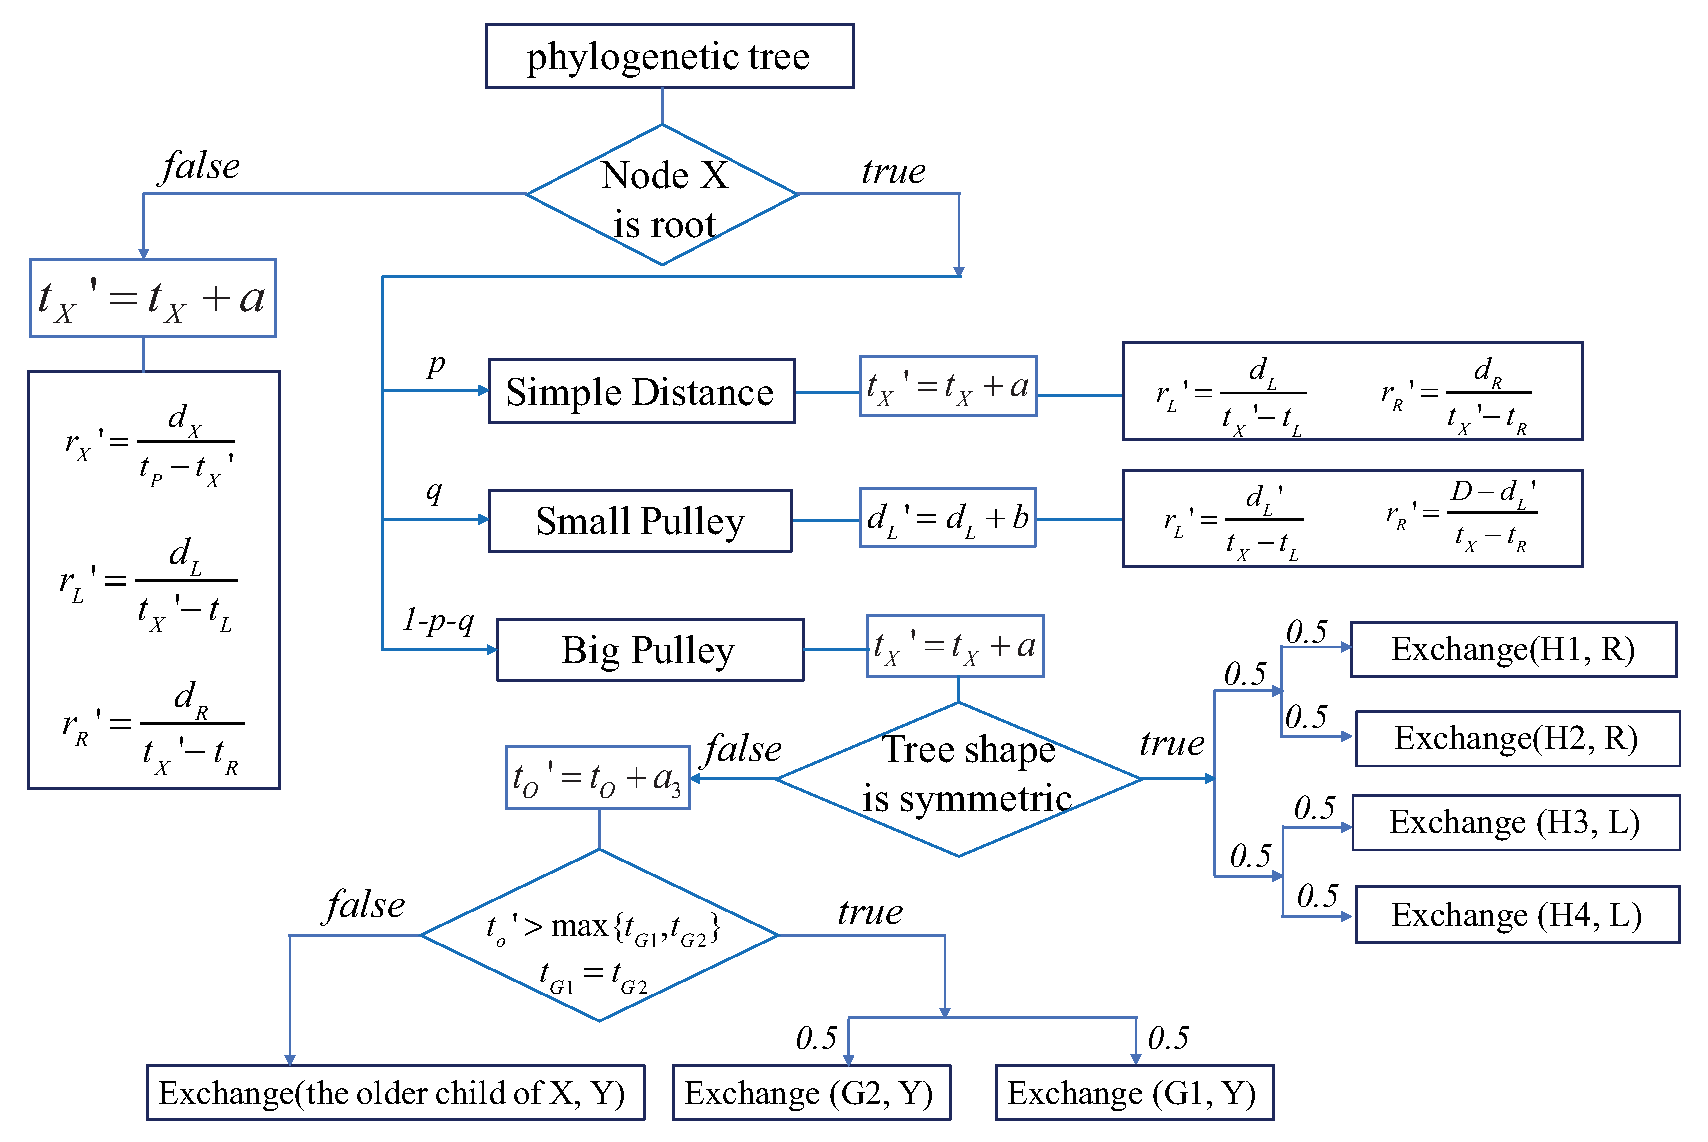
\includegraphics[width=12cm]{Fig01-flowchart.eps}\\
\caption{\csentence{The flow chart of the Constant Distance operator.}}
\label{flowchart}
\end{figure}

\begin{figure}[h!]
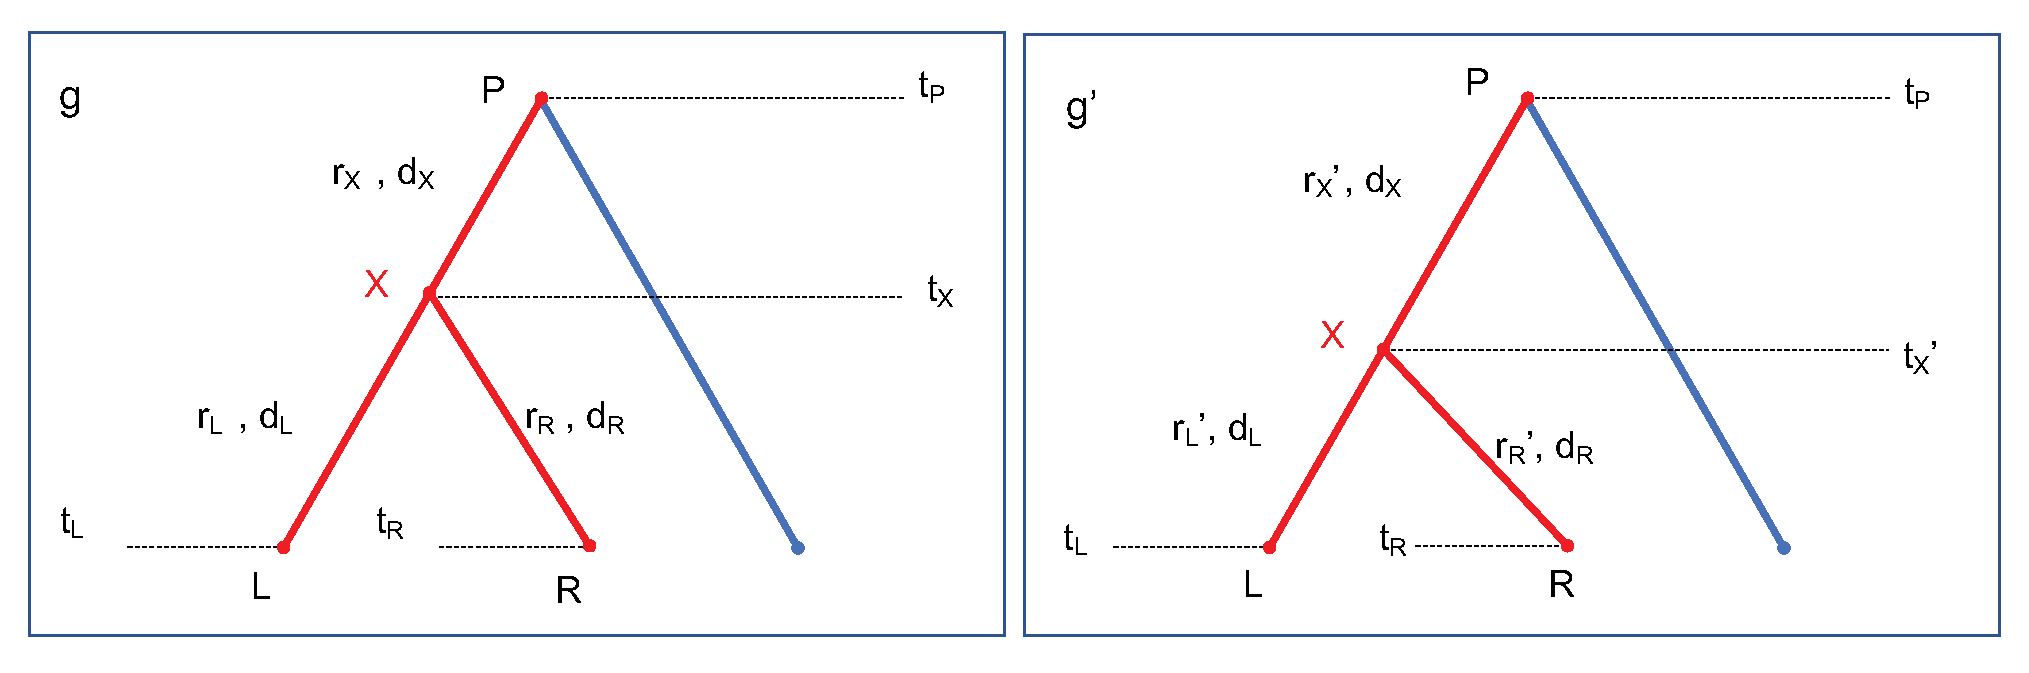
\includegraphics[width=12cm]{Fig02-internalnodes.eps}\\
\caption{\csentence{Illustration of the operation on an internal node.}
             The operator proposes a tree ${g_{in}}'$ based on tree $g_{in}$, during which $d_i$, $d_j$, $d_k$ are kept constant.}
\label{internalnodes}
\end{figure}

\begin{figure}[h!]
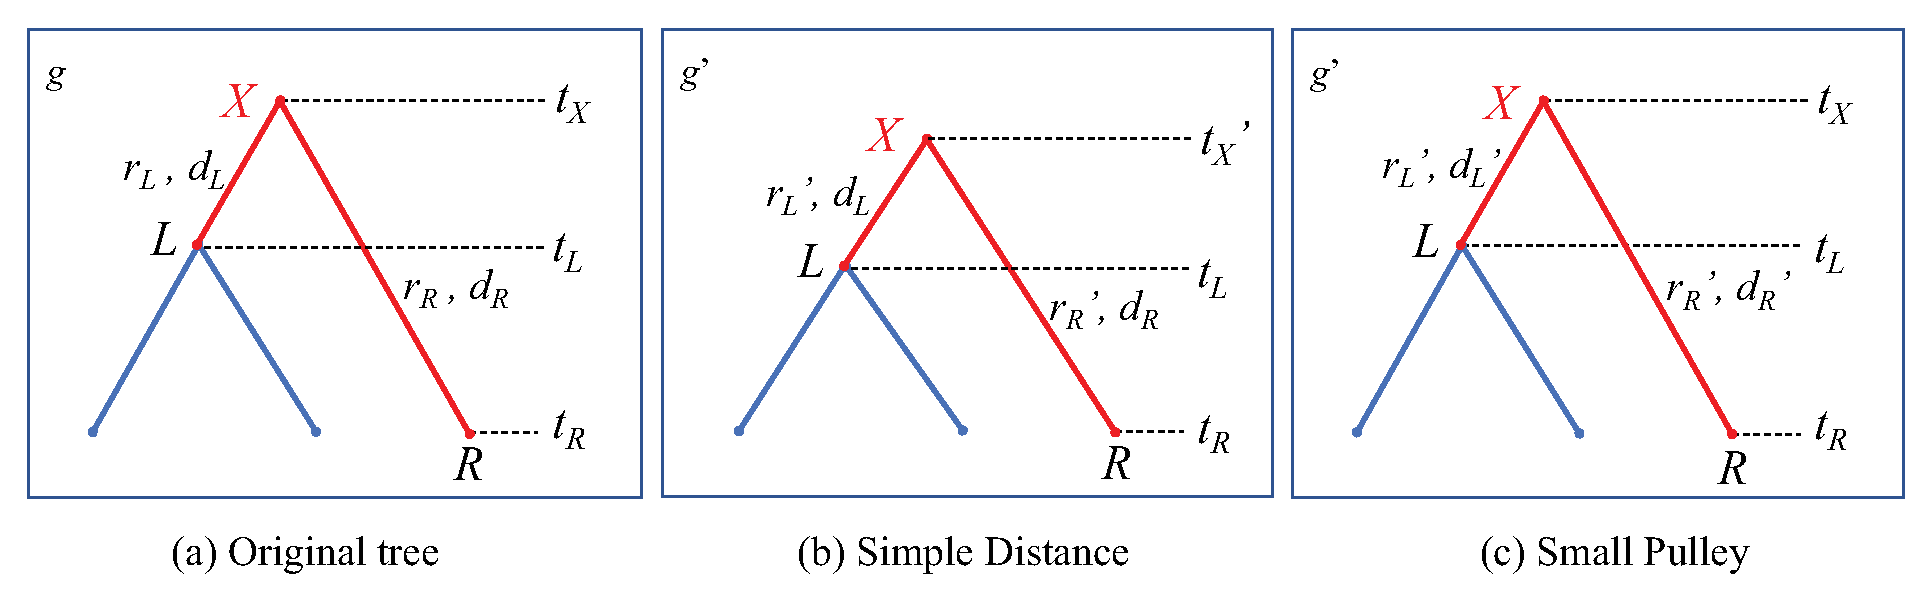
\includegraphics[width=12cm]{Fig03-rootstrategy.eps}\\
\caption{\csentence{Illustration of Simple Distance and Small Pulley sub-moves.}
             Simple Distance proposes ${g_{r1}}'$ and keeps $d_i$, $d_x$ constant. Small Pulley proposes ${g_{r2}}'$ and ${d_i} + {d_x}$ remains constant.}
\label{simpledistance}
\end{figure}


\begin{figure}[h!]
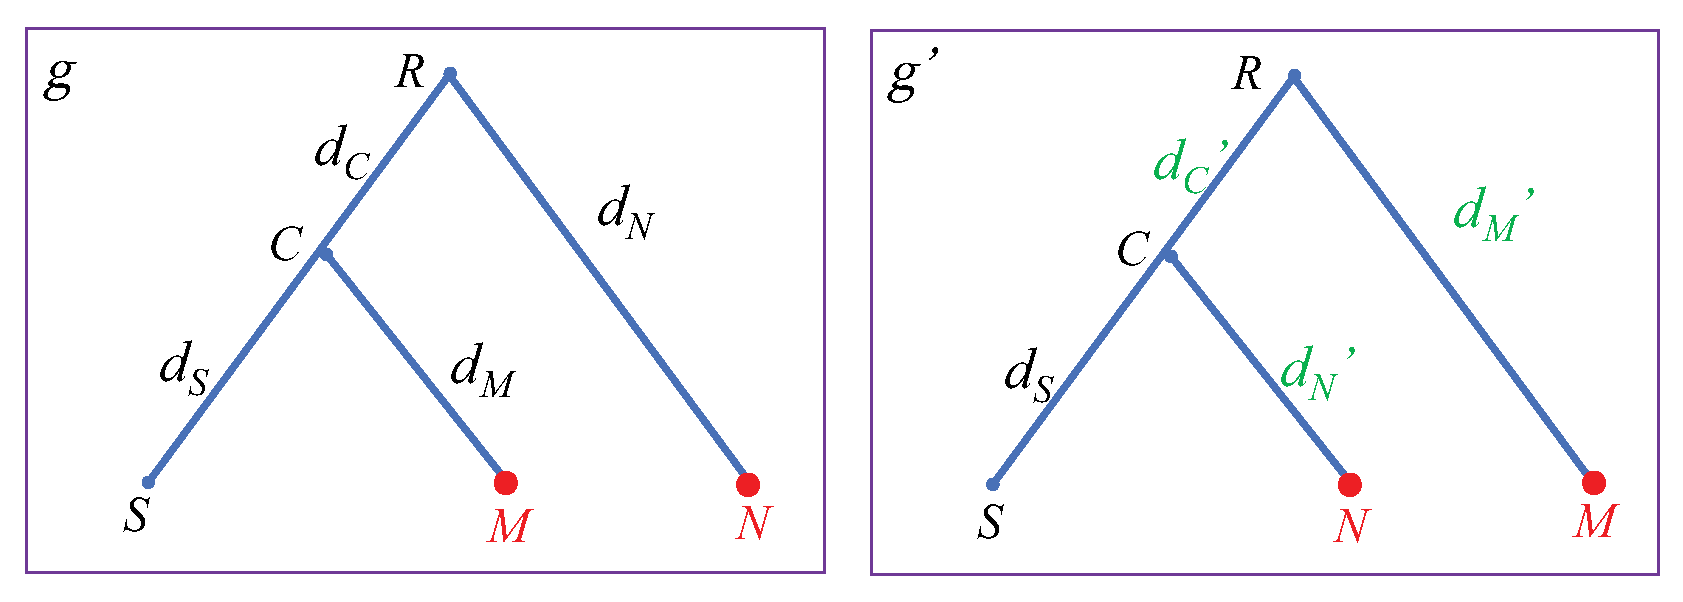
\includegraphics[width=12cm]{Fig04-exchangemethod.eps}\\
\caption{\csentence{Illustration of \textit{Exchange (\textbf{M},\textbf{N})} method.}
             This method is applied to tree $g$ and proposes $g'$ by swapping \textbf{M} and \textbf{N}, so that the three distances are adjusted to maintain the distances among \textbf{S}, \textbf{M} and \textbf{N}. That is, ${d_C}' = {d_C} + b$, ${d_N}' = d_C + d_N$ and ${d_M}' = d_{M} - {d_C}'$, where $b \sim U[ - v, + v]$.}
\label{exchangemethod}
\end{figure}

\begin{figure}[h!]
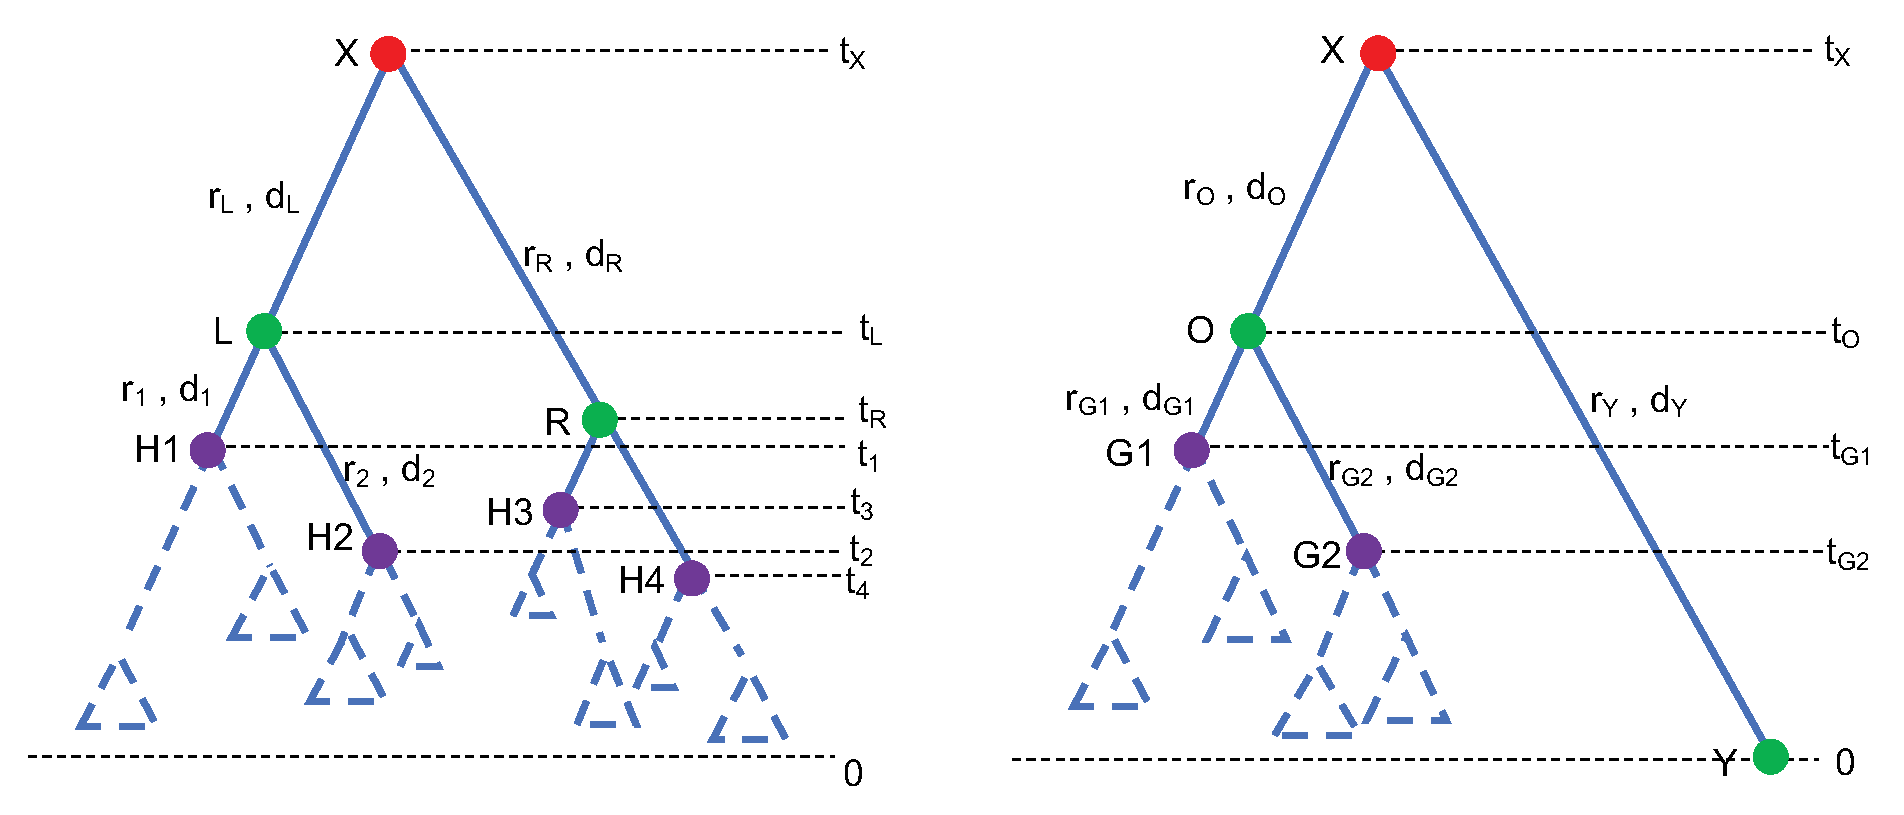
\includegraphics[width=12cm]{Fig05-treeshape.eps}\\
\caption{\csentence{Two different tree shapes.}
             The symmetric tree is on the left and the asymmetric tree is on the right. The dashed triangles represent the potential subtrees rooted at the nodes.}
\label{treeshape}
\end{figure}

\begin{figure}[h!]
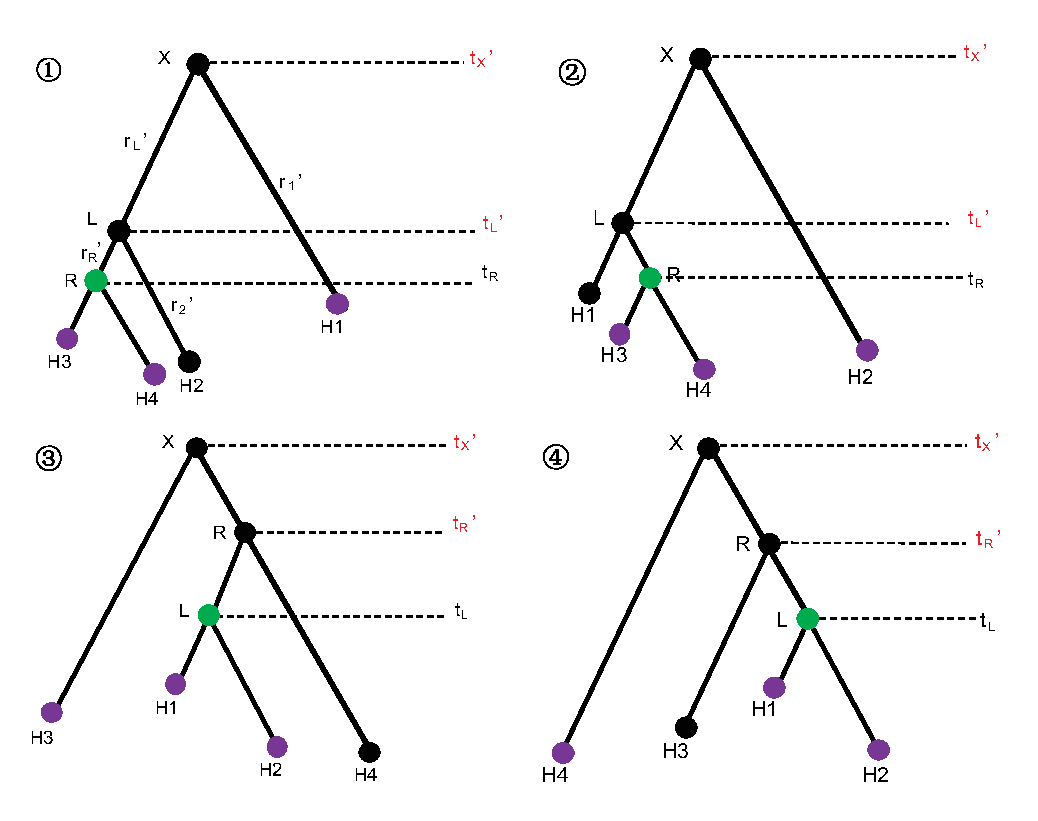
\includegraphics[width=12cm]{Fig06-symmetric.eps}\\
\caption{\csentence{Illustration of operations on the symmetric tree in Figure \ref{treeshape}.}
             The proposed operator will propose one of the four possible trees, each with 0.25 probability.}
\label{symmetric}
\end{figure}

\begin{figure}[h!]
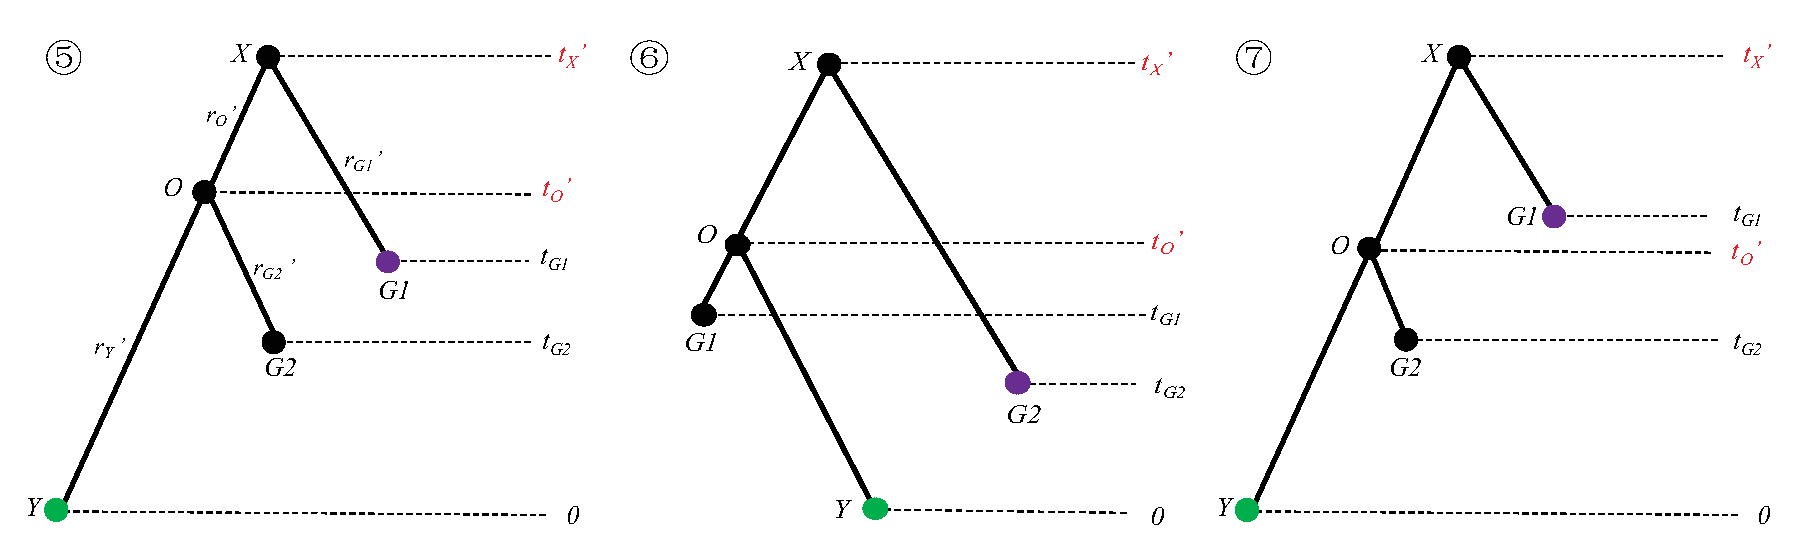
\includegraphics[width=12cm]{Fig07-asymmetric.eps}\\
\caption{\csentence{Illustration of operations on the asymmetric tree in Figure \ref{treeshape}.}
             The proposed operator will propose one of the three possible trees. If ${t_o}' < t_{G1}$, \textcircled7 has 1 probability, otherwise \textcircled5 and \textcircled6 have 0.5 probability each.}
\label{asymmetric}
\end{figure}

\begin{figure}[h!]
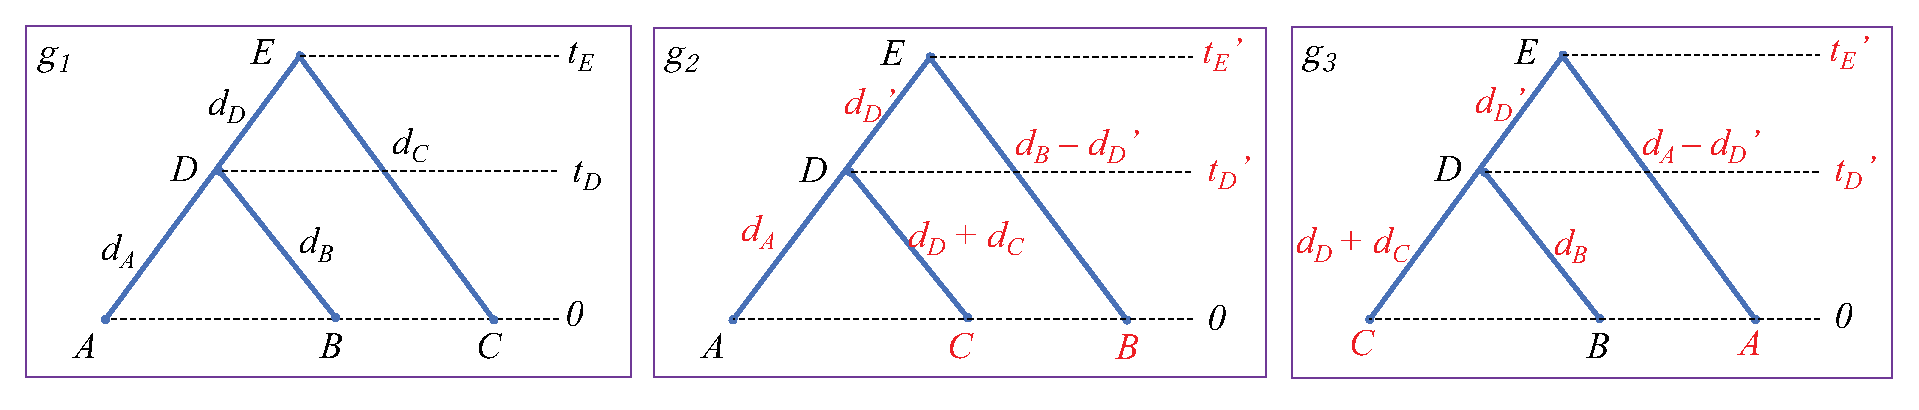
\includegraphics[width=12cm]{Fig08-sampleprior.eps}\\
\caption{\csentence{The illustration of sampling from prior.}
             $g_1$ is set to be the original tree where an MCMC chain starts. When testing Big Pulley, the proposed operator samples the trees among $g_1$, $g_2$ and $g_3$.}
\label{sampleprior}
\end{figure}

\begin{figure}[h!]
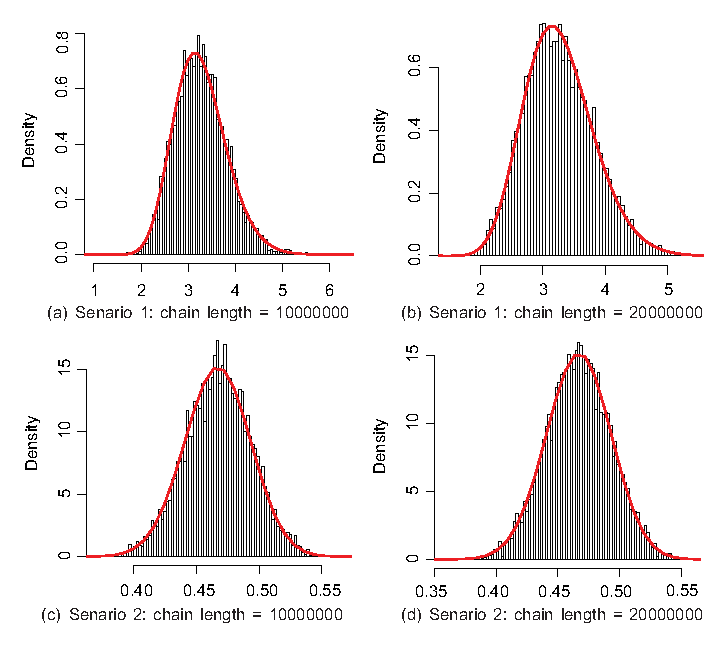
\includegraphics[width=12cm]{Fig09-testinternalnode.eps}\\
\caption{ \csentence{Sampled parameters in tests of internal nodes.}
             The horizontal axis represents the node time of D in Figure \ref{sampleprior}. The two scenarios sample two trees with different distances specified in Table \ref{ini_inter}.}
\label{res_int}
\end{figure}

\begin{figure}[h!]
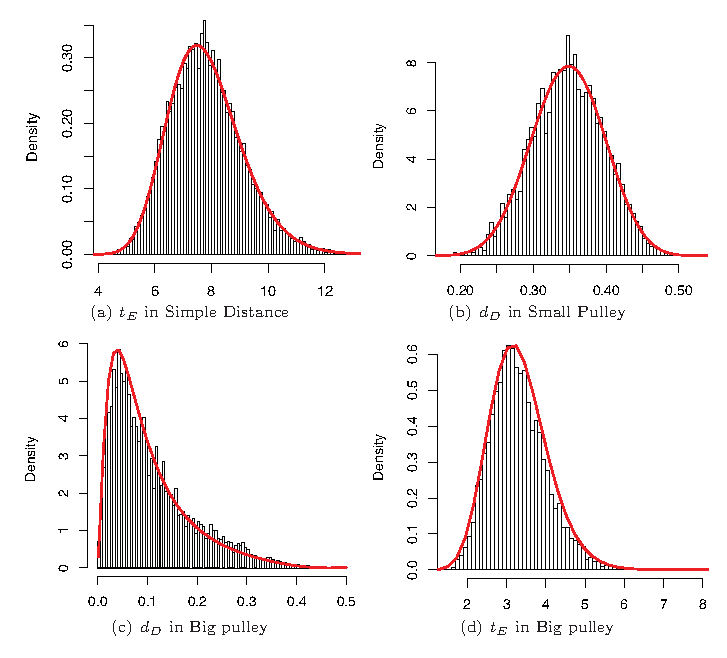
\includegraphics[width=12cm]{Fig10-testroot.eps}\\
\caption{\csentence{Sampled parameters in test of the root.}
             For the trees in Figure \ref{sampleprior}, Simple Distance samples the root time $t_E$ only, Small Pulley samples the distance $d_D$ only, and Big Pulley samples $t_E$, $t_D$, $d_D$. To make it simple, $t_E$ and $d_D$ are compared.}
\label{res_roo1}
\end{figure}

\begin{figure}[h!]
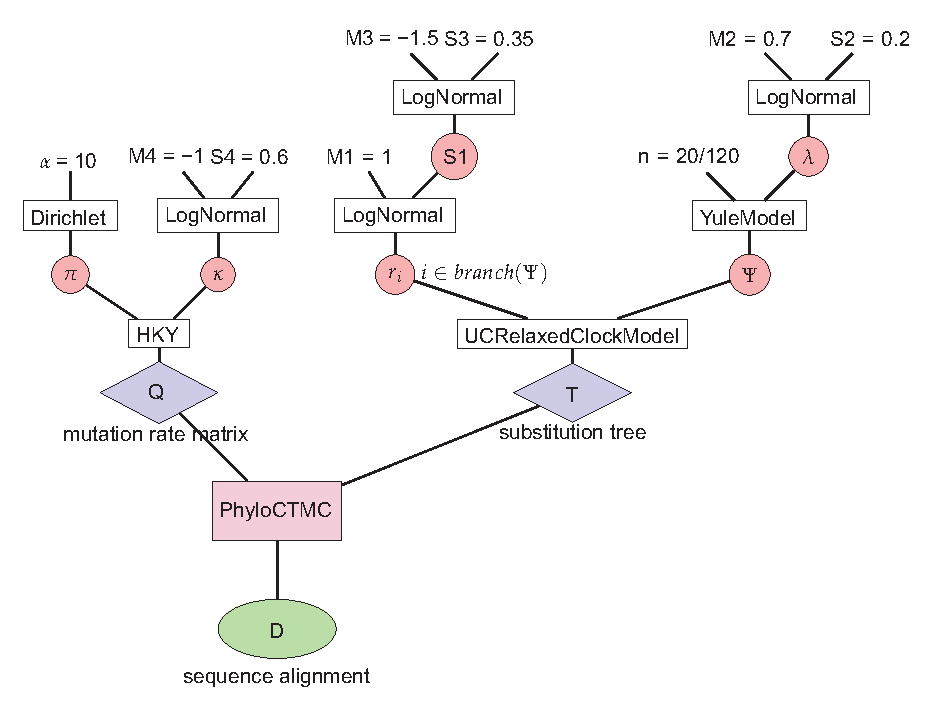
\includegraphics[width=12cm]{Fig11-modelvalidation.eps}\\
\caption{\csentence{The models and prior distributions to simulate the sequence data.}
             The sequence alignment is simulated through a phylogenetic continuous-time Markov Chain that consists of a substitution model (HKY) and an uncorrelated relaxed clock model. The random variables in HKY model construct the mutation rate matrix, including frequency and ratio. The rates and time trees specified by a Yule model construct the substitution tree. The standard deviation of rates and the birth rate in Yule model are both random variables following LogNormal distributions.}
\label{modelvalidation}
\end{figure}

\begin{figure}[h!]
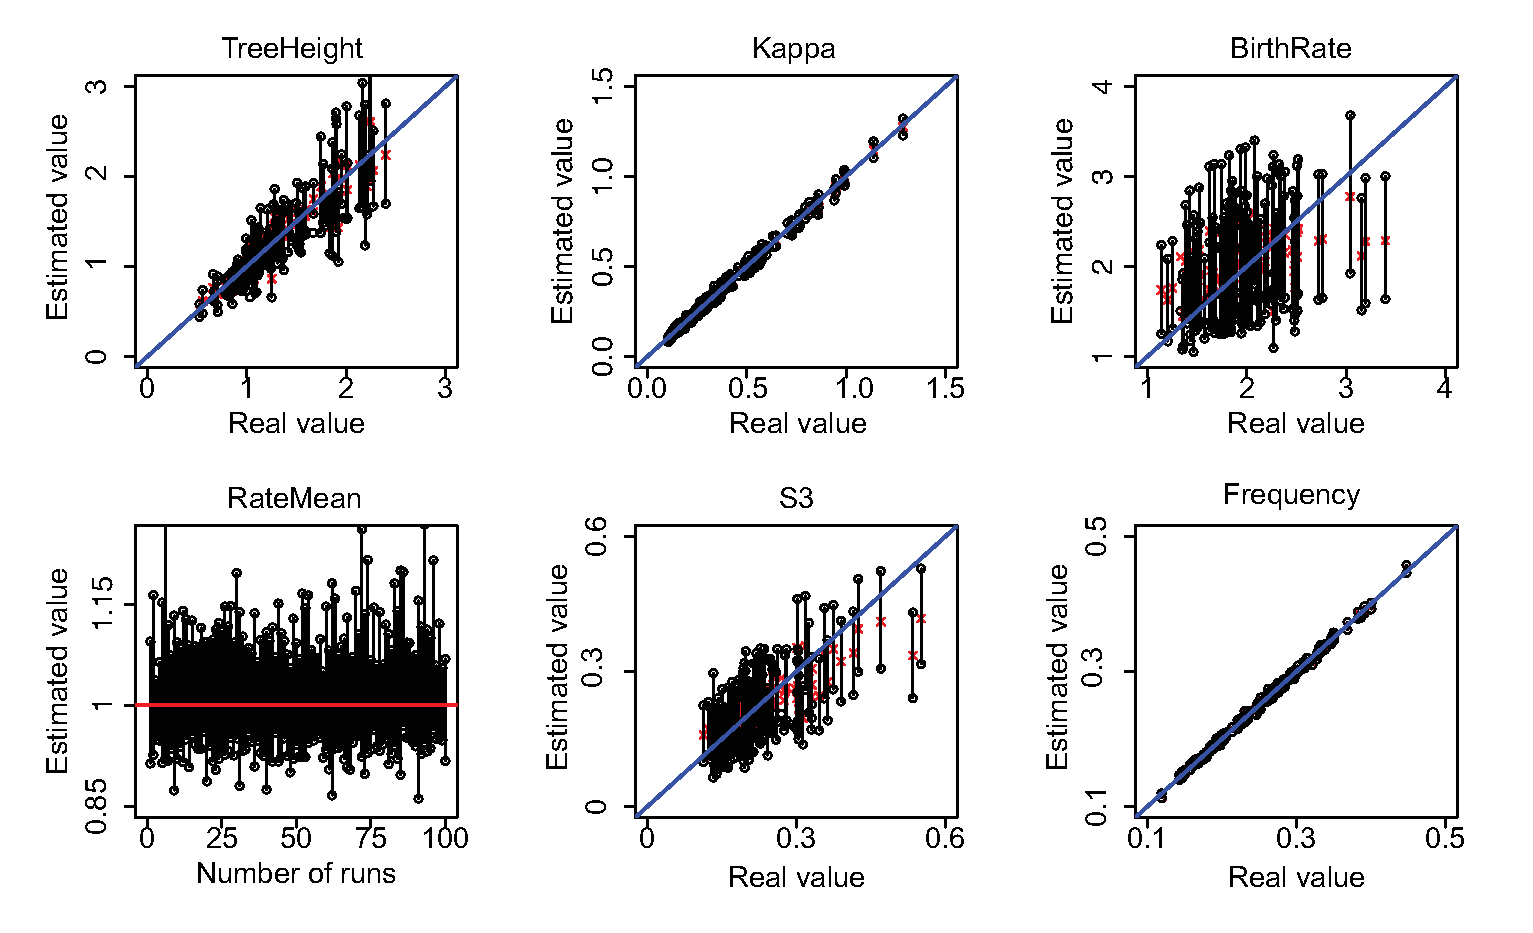
\includegraphics[width=12cm]{Fig12-smalltree.eps}\\
\caption{\csentence{Comparing the sampled parameters in simulation study with 20 taxa.}
             The red crossings represent the coordinates of real and estimated value. The vertical lines with circles show the 95\% HPD of the sampled parameters. The blue lines indicate that the estimated value is equal to the real value. The red line represents the fixed value of rate mean.}
\label{SmallTree}
\end{figure}

\begin{figure}[h!]
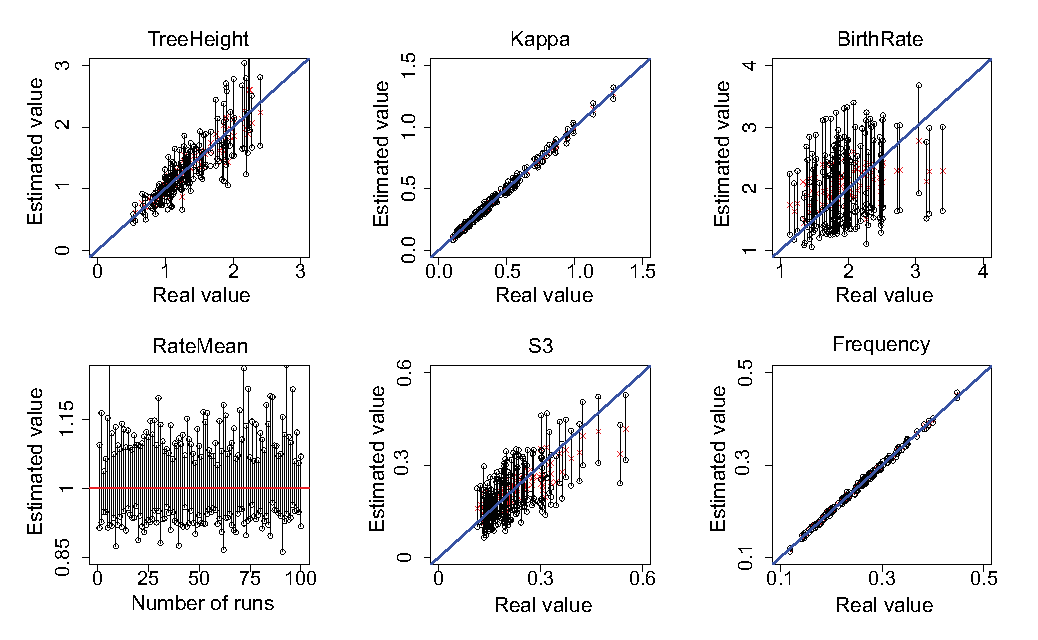
\includegraphics[width=12cm]{Fig13-largetree.eps}\\
\caption{\csentence{Comparing the sampled parameters in simulation study with 120 taxa.}
             }
\label{LargeTree}
\end{figure}

\begin{figure}[h!]
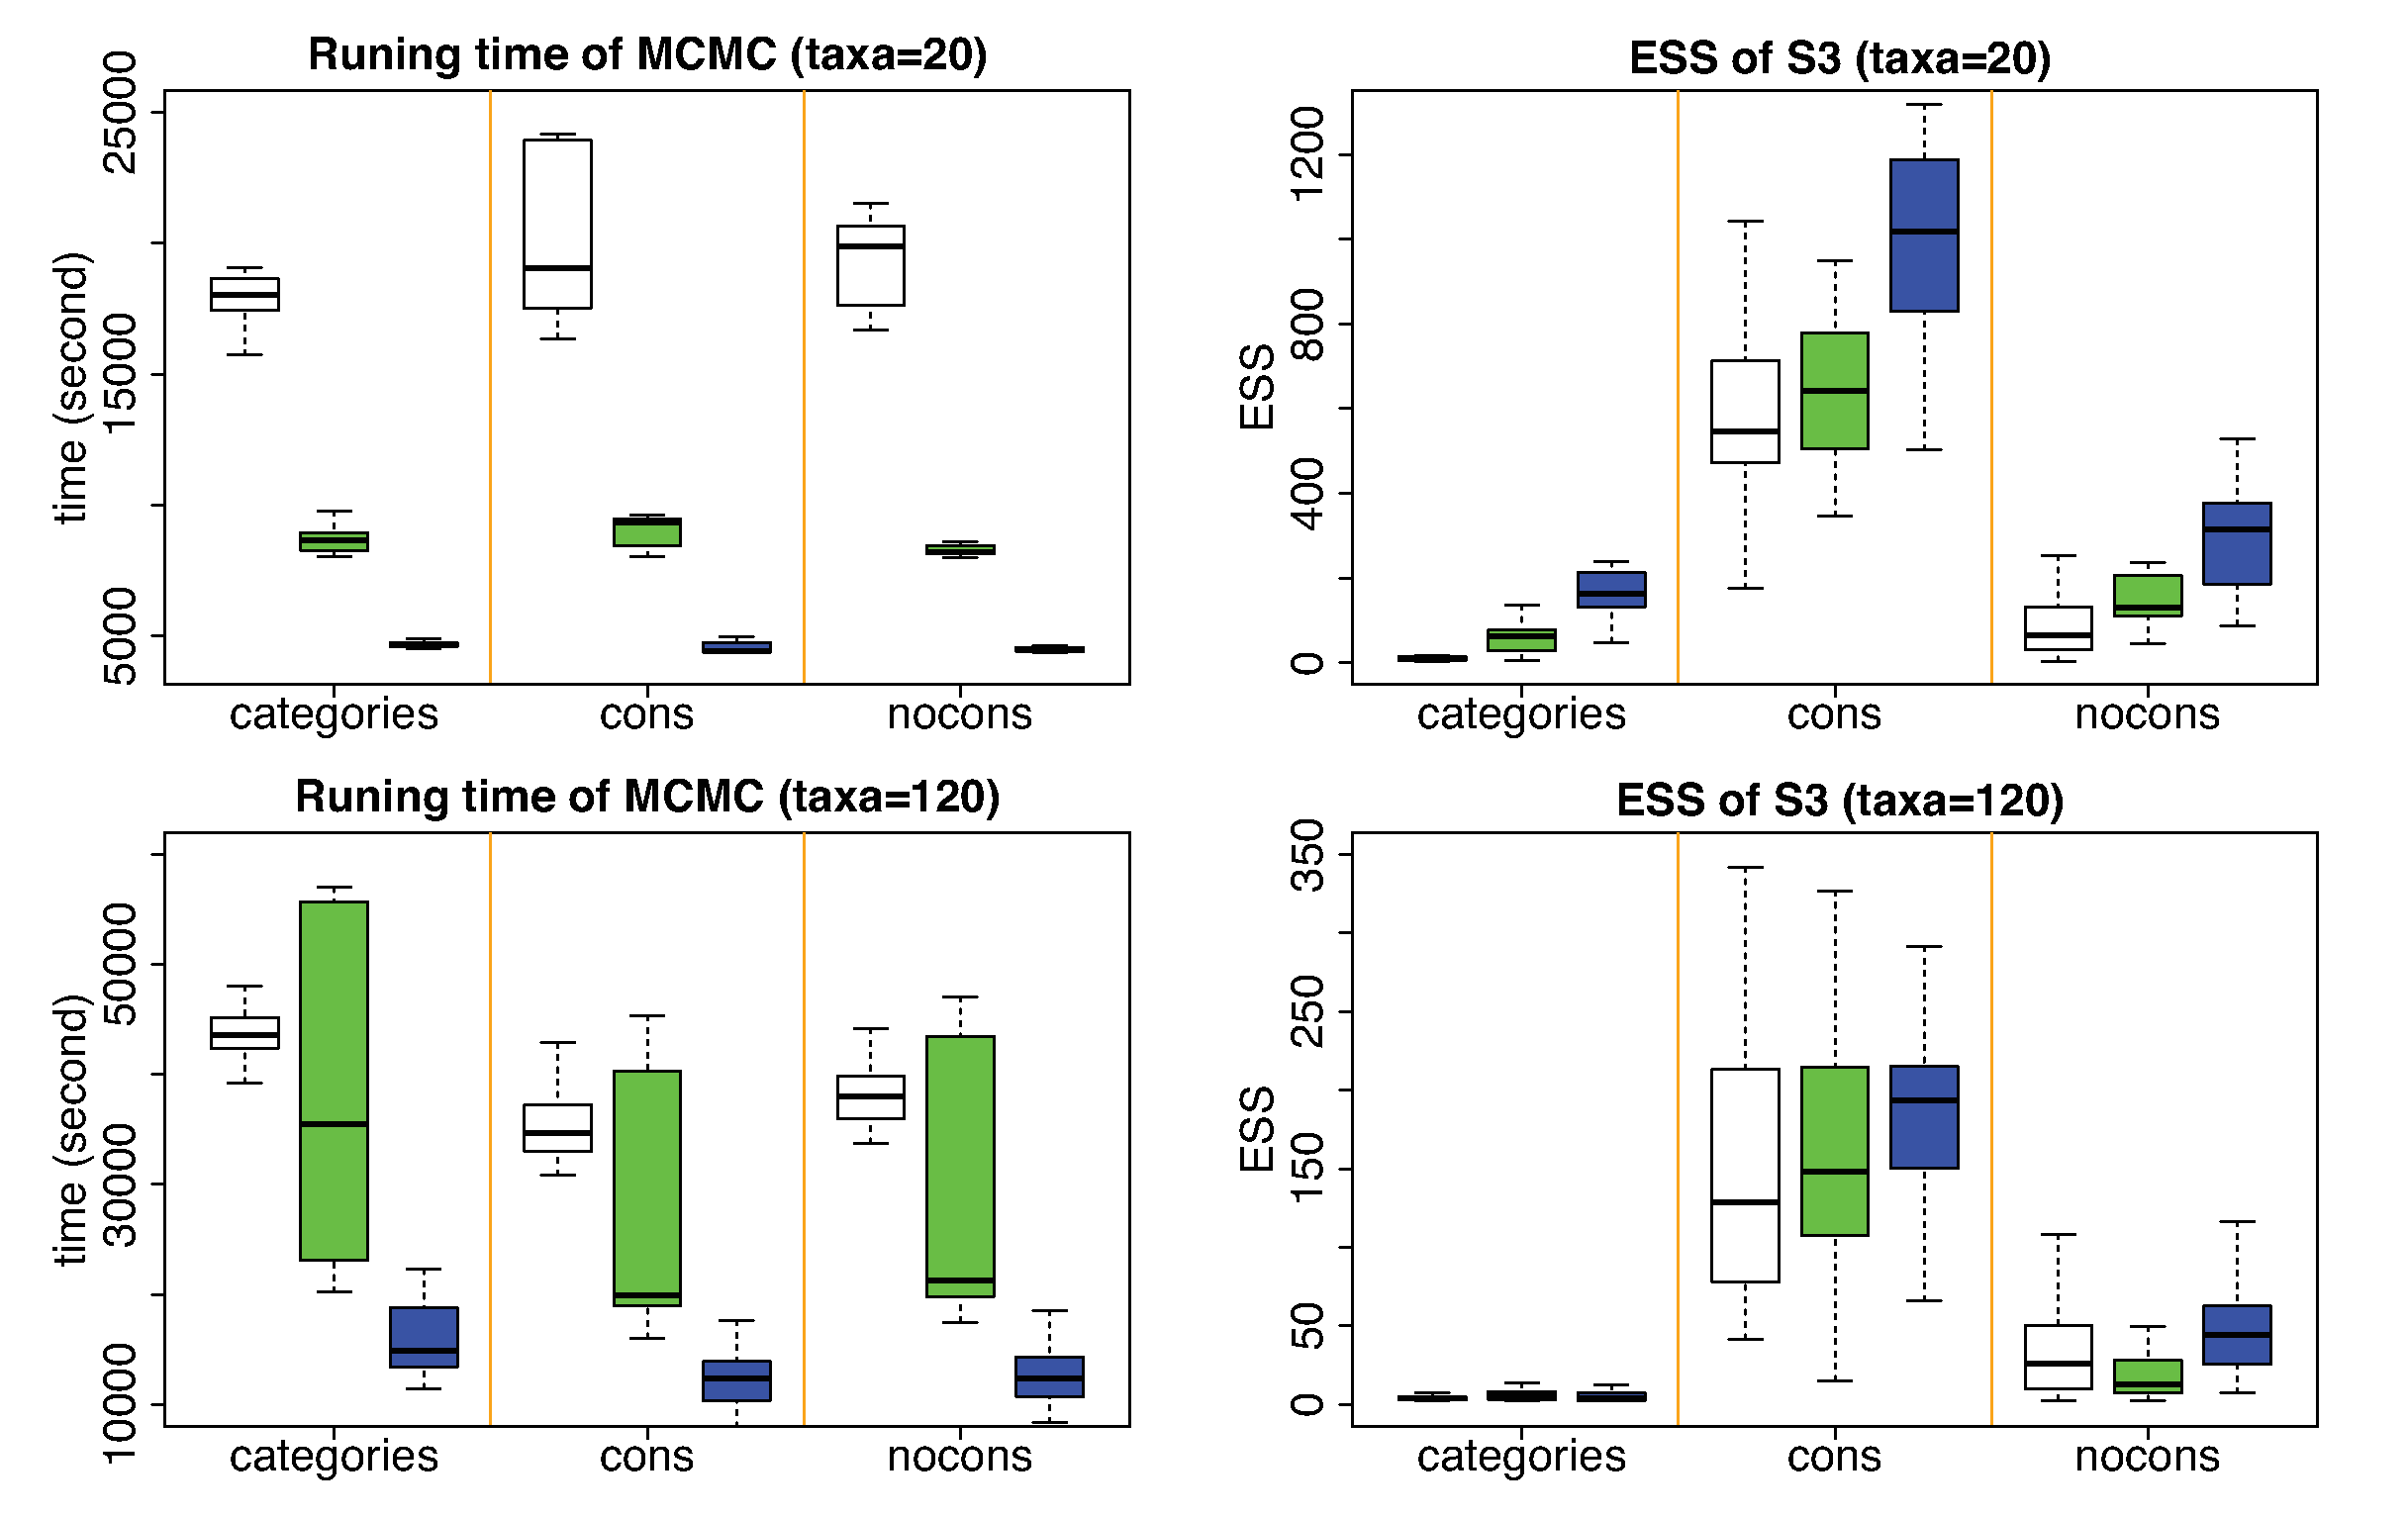
\includegraphics[width=12cm]{Fig14-efficiency.eps}\\
\caption{\csentence{Comparison of ESS and running time using simulated data.}
             The term long, medium and short represent the length of sequence with 20 thousand, 10 thousand and 5 thousand respectively.}
\label{eff_comp}
\end{figure}

\begin{figure}[h!]
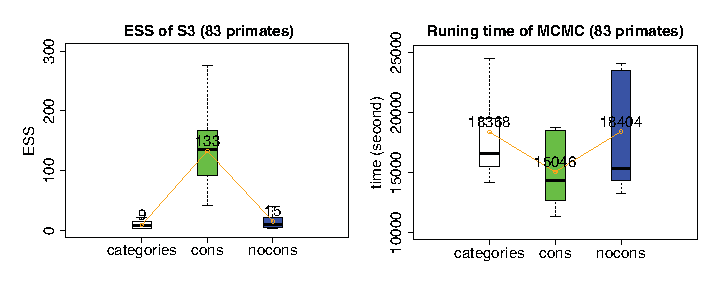
\includegraphics[width=12cm]{Fig15-primates.eps}\\
\caption{\csentence{Comparison of ESS and running time using primates data.}
             The orange curve links the mean values of each boxplot and the values are shown on the left of the boxplot.}
\label{eff_comp2}
\end{figure}

\begin{figure}[h!]
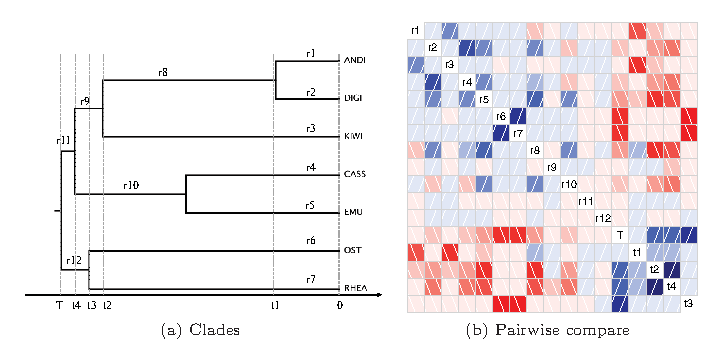
\includegraphics[width=12cm]{Fig16-correlation.eps}\\
\caption{\csentence{Correlation between rates and node times in the ratites tree.}
             Blue indicates the positive relation and red indicates the negative relation. The darker the colour is, the stronger the relation tends to be.}
\label{correlation}
\end{figure}

\begin{figure}[h!]
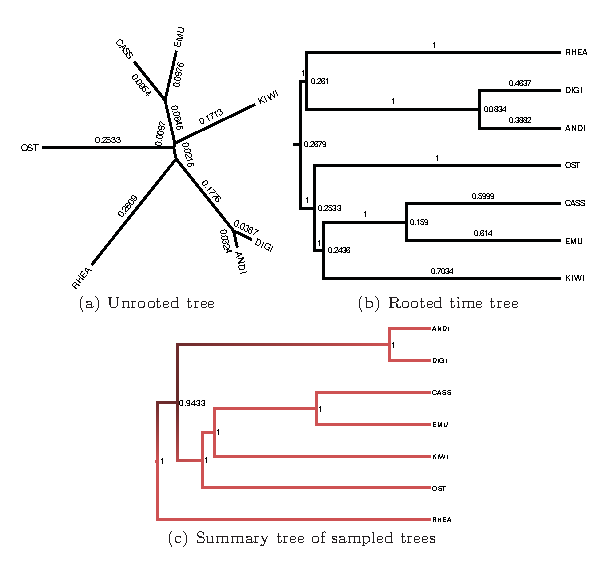
\includegraphics[width=12cm]{Fig17-fixedtree.eps}\\
\caption{\csentence{Illustration of sampling a fixed unrooted tree.}
            The unrooted tree is obtained from the ratites data set \cite{cooper2001complete}. The colour of branches from green to red indicates the rates increasing from small to large. The blue bars at represents the 95\% HPD of the node times. And the numbers besides the blue bars are the posterior values at the corresponding nodes.}
\label{withoutdata}
\end{figure}

\clearpage
%%%%%%%%%%%%%%%%%%%%%%%%%%%%%%%%%%%
%%                               %%
%% Tables                        %%
%%                               %%
%%%%%%%%%%%%%%%%%%%%%%%%%%%%%%%%%%%
%% Use of \listoftables is discouraged.
%%
\section*{Tables}
\begin{table}[h!]
  \centering
\begin{tabular}{c|cccc|c|c|cccc}
  \hline
&\multicolumn{4}{c|}{genetic distances (fixed)}&$t_D$&$t_E$&\multicolumn{4}{c}{initial rates}\\
&${d_j}$&${d_k}$&${d_x}$&${d_i}$&initial&(fixed)&${r_j}$&${r_k}$&${r_x}$&${r_i}$\\
\hline
Scenario 1&0.1&0.2&0.4&0.27&1&10&0.1&0.2&0.04&0.03\\
\hline
Scenario 2&0.4&0.8&2.4&1.6&0.4&0.8&1&2&3&4\\
  \hline
\end{tabular}
\caption{Initial settings for testing operations on internal nodes}\label{ini_inter}
\end{table}

\begin{table}[h!]
  \centering
\begin{tabular}{c|c|ccc|ccc|c}
  \hline
&\multirow{2}*{Chain Length}&\multicolumn{3}{c|}{Sample from MCMC}&\multicolumn{3}{c|}{Integral curve}&Plot\\
&~&Mean&Err&StdEv&Mean&Err&StdEv&\\
\hline
\multirow{2}*{Senario 1}&10000000&3.2727&8.3e-3&0.5467&\multirow{2}*{3.2669}&\multirow{2}*{1.3e-06}&\multirow{2}*{0.5553}&Figure \ref{res_int}(a)\\
~&20000000&3.271&6.1e-3&0.5616&~&~&~&Figure \ref{res_int}(b)\\
\hline
\multirow{2}*{Senario 2}&10000000&0.4677&3.9e-04&0.0265&\multirow{2}*{0.4667}&\multirow{2}*{3.5e-05}&\multirow{2}*{0.0262}&Figure \ref{res_int}(c)\\
~&20000000&0.4672&2.8e-04&0.0262&~&~&~&Figure \ref{res_int}(d)\\
  \hline
\end{tabular}
\caption{Results of sampling the internal node}\label{res_inter}
\end{table}

\begin{table}[h!]
  \centering
\begin{tabular}{c|cccc|c|c|cccc}
  \hline
\multirow{2}*{Strategy}&\multicolumn{4}{c|}{genetic distances}&\multirow{2}*{$t_D$}&\multirow{2}*{$t_E$}&\multicolumn{4}{c}{initial rates}\\
~&${d_j}$&${d_k}$&${d_x}$&${d_i}$&~&~&${r_j}$&${r_k}$&${r_x}$&${r_i}$\\
\hline
Simple Distance&0.1&0.2&0.4&0.27&1&10&0.1&0.2&0.04&0.03\\
Small Pulley&0.1&0.2&\multicolumn{2}{|c|}{0.67}&1&10&0.1&0.2&0.04&0.03\\
Big Pulley&0.5&0.5&\multicolumn{2}{|c|}{0.5}&5&10&0.1&0.1&0.03&0.04\\
  \hline
\end{tabular}
\caption{Initial settings for operations on the root}\label{ini_sim}
\end{table}

\begin{table}[h!]
\centering
\begin{tabular}{c|c|cc|cc|cc}
  \hline
\multirow{2}*{Strategy}&\multirow{2}*{Variable}&\multicolumn{2}{c|}{Sample from MCMC}&\multicolumn{2}{c|}{Integral curve}&\multirow{2}*{Plot}\\
&~&Mean&StdEv&Mean&StdEv&\\
\hline
Simple Distance&$t_E$&7.8081&1.2884&7.8187&1.2992&Figure \ref{res_roo1}(a)\\
\hline
Small Pulley&${d_i}$&0.3480&0.0492&0.3476&0.0494&Figure \ref{res_roo1}(b)\\
\hline
\multirow{2}*{Big Pulley}&${d_i}$&0.1016&0.0766&0.0960&0.0760&Figure \ref{res_roo1}(c)\\
~&$t_E$&3.3017&0.6908&3.3095&0.6912&Figure \ref{res_roo1}(d)\\
\hline
\end{tabular}
\caption{Results of sampling the root}\label{res_sma}
\end{table}

\begin{table}[h!]
  \centering
\begin{tabular}{cccccccc}
\hline
&BirthRate&TreeHeight&RateMean&UcldStdev&Kappa&Frequency\\
\hline
20 taxa&93&98&100&95&100&100\\
120 taxa&100&98&85&94&100&100\\
\hline
\end{tabular}
\caption{Number of real values lying in the 95\% HPD in Figure \ref{SmallTree} and Figure \ref{LargeTree} }\label{num_hpd}
\end{table}

\begin{table}[h!]
  \centering
\begin{tabular}{cc|cc|cc|cc}
\hline
&&\multicolumn{2}{c|}{ESS of of analysis}&\multicolumn{2}{c|}{Running time(second)}&\multicolumn{2}{c}{ESS per hour}\\
\hline
&Length&20 taxa&120 taxa&20 taxa&120 taxa&20 taxa&120 taxa\\
categories&20000&13&4&18635&44155&2.47&0.36\\
&10000&58&6&8660&36406&24.11&0.62\\
&5000&171&8&4690&15956&131.09&1.89\\
Average&&81&6&10662&32172&27.19&0.71\\
\hline
cons&20000&616&147&20207&35406&109.72&14.92\\
&10000&646&161&8967&25589&259.24&22.68\\
&5000&993&186&4581&12487&780.50&53.70\\
Average&&752&165&11252&24494&240.24&24.21\\
\hline
nocons&20000&86&63&19344&38245&16.09&5.91\\
&10000&153&20&8361&30521&65.83&2.31\\
&5000&296&48&4499&12940&237.04&13.22\\
Average&&179&43&10735&27236&59.87&5.72\\
\hline
\end{tabular}
\caption{Summary of ESS and running time using simulated data}\label{eff_comp1}
\end{table}
%%%%%%%%%%%%%%%%%%%%%%%%%%%%%%%%%%%
%%                               %%
%% Additional Files              %%
%%                               %%
%%%%%%%%%%%%%%%%%%%%%%%%%%%%%%%%%%%
\clearpage
\newpage
\section*{Appendix}
\subsection*{The Green ratio}
When developing an operator for MCMC, the proposal function must be reversible. In other words, the probability that the operator propose a new state from the current state is required to be equal to the probability that the proposed state goes back to current state. To be specific, let ${\pi (x)}$ be the target probability distribution and $p(x, x')$ be the transition kernel in the continuous Markov chain. The reversibility condition requires that ${\pi (x)}{p(x, x')} = {\pi (x')}{p(x', x)}$. And an operator provides a proposal $q(x, x')$ with some probability $\alpha(x, x')$ that the proposal is accepted. Thus, the reversibility condition is rewritten as ${\pi (x)}{q(x, x')}{\alpha(x, x')} = {\pi (x')}{q(x', x)}{\alpha(x', x)}$.

Considering the subspace $\varphi_1$ on $x$ and subspace $\varphi_2$ on $x'$, it is assumed that there is a symmetric measure on the combined parametric space $\varphi = {\varphi_1} \times {\varphi_2}$, so that ${\pi (x)}{q(x, x')}$ has a density with respect to a single measure on $\varphi$. Then, Green suggested that the reversibility condition should be satisfied by detailed balance \cite{green1995reversible}, as represented by Equation (\ref{balance}). And according to Peskun' proof, it is optimal to take Equation (\ref{Ratio}) as the acceptance probability to retain the detailed balance \cite{peskun1973optimum}.

\begin{equation}\label{balance}
\int_A {\pi (x) d_x} {\int_B  {q(x, x')}{\alpha(x, x')} d_x}  = \int_B {\pi (x') d_{x'}}{\int_A {q(x', x)}{\alpha(x', x)} d_{x'}} \text{,}
\end{equation}
where $A \in {\varphi_1}$ and $B \in  {\varphi_2}$ are two Borel sets. ${q(x, x')}$ denotes the probability that the operator proposes a new state $x'$ given the current state $x$.

\begin{equation}\label{Ratio}
{\alpha_H}(x, x') = \min \left\{ {1,\frac{{\pi (x'){p}(x',x)}}{{\pi (x){p}(x,x')}}} \right\} \text{,}
\end{equation}
where ${p(x',dx)}/{p(x,dx')}$ is known as the Hastings ratio.

However, for operators that do not have a symmetric measure, it is necessary to include the Jacobian matrix ${\mathbf{J}}$  in order to deal with the dimension matching problem, as is discussed in Green's paper \cite{green1995reversible}. In this case, Equation (\ref{Ratio}) is extended, as is shown in Equation (\ref{Green}).
\begin{equation}\label{Green}
{\alpha_G}(x, x') = \min \left\{ {1,\frac{{\pi (x'){p}(x',x)}}{{\pi (x){p}(x,x')}}}\left|{\mathbf{J}}\right| \right\} \text{,}
\end{equation}
where ${\mathbf{J}} = {\nabla h(x, x')}$ represents a vector differential matrix of deterministic function $h$. $\alpha = \frac{{p}(x',x)}{{p}(x,x')}\left|{\mathbf{J}}\right|$ is defined as the Green ratio, and ${\mathbf{J}}$ ensures that the proposal have a symmetric measure on each subspace in state $x$ and $x'$.

\subsection*{Calculating the Green ratio for operations on internal nodes}
The Constant Distance Operator firstly proposes a new time for the randomly selected internal node (Equation (\ref{in_HR1.1})), and then proposes three rates by the original distances and new node times(Equation (\ref{in_HR1.2})$\sim$Equation (\ref{in_HR1.3})).
\begin{subequations}\label{in_HR1}
\begin{equation}\label{in_HR1.1}
{f_1}:{{\text{t}}_X}{\text{'  =  }}{{\text{t}}_X}{\text{  +  a}}
\end{equation}
\begin{equation}\label{in_HR1.2}
{f_2}:{r_X}' = \frac{{{r_X} \times ({t_P} - {t_X})}}{{{t_P} - {t_X}'}}
\end{equation}
\begin{equation}
{f_3}:{r_L}' = \frac{{{r_L} \times ({t_X} - {t_L})}}{{{t_X}' - {t_L}}}
\end{equation}
\begin{equation}\label{in_HR1.3}
{f_4}:{r_R}' = \frac{{{r_R} \times ({t_X} - {t_2})}}{{{t_X}' - {t_R}}}
\end{equation}
\end{subequations}

Substituting Equation (\ref{in_HR1}) in the Jacobian matrix ${{\mathbf{J}}_1}$ (Equation (\ref{JacobianMatrix})), we can get Equation (\ref{in_HR2}), so that the determinant of ${{\mathbf{J}}_1}$ can be obtained by Equation (\ref{in_HR3}).
\begin{equation}\label{in_HR2}
{{\mathbf{J}}_1} = \left[ {\begin{array}{*{20}{c}}
  1&0&0&0 \\
  {\frac{{ - {r_X}}}{{{t_P} - {t_X}'}}}&{\frac{{{t_P} - {t_X}}}{{{t_P} - {t_X}'}}}&0&0 \\
  {\frac{{{r_L}}}{{{t_X}' - {t_L}}}}&0&{\frac{{{t_X} - {t_L}}}{{{t_X}' - {t_L}}}}&0 \\
  {\frac{{{r_R}}}{{{t_X}' - {t_R}}}}&0&0&{\frac{{{t_X} - {t_R}}}{{{t_X}' - {t_R}}}}
\end{array}} \right]
\end{equation}
\begin{equation}\label{in_HR3}
\begin{aligned}
\left| {{{\mathbf{J}}_1}} \right| &= 1 \times \left| {\begin{array}{*{20}{c}}
  {\frac{{{t_P} - {t_X}}}{{{t_P} - {t_X}'}}}&0&0 \\
  0&{\frac{{{t_X} - {t_L}}}{{{t_X}' - {t_L}}}}&0 \\
  0&0&{\frac{{{t_X} - {t_R}}}{{{t_X}' - {t_R}}}}
\end{array}} \right| \\&= \frac{{{t_P} - {t_X}}}{{{t_P} - {t_X}'}} \times \left| {\begin{array}{*{20}{c}}
  {\frac{{{t_X} - {t_L}}}{{{t_X}' - {t_L}}}}&0 \\
  0&{\frac{{{t_X} - {t_R}}}{{{t_X}' - {t_R}}}}
\end{array}} \right| \\&= \frac{{{t_P} - {t_X}}}{{{t_P} - {t_X}'}} \times \frac{{{t_X} - {t_L}}}{{{t_X}' - {t_L}}} \times \frac{{{t_X} - {t_R}}}{{{t_X}' - {t_R}}}
\end{aligned}
\end{equation}

\subsection*{Calculating the Green ratio for Simple Distance}
Simple Distance proposes two rates by using Equation (\ref{SD_HR1.2}) and Equation (\ref{SD_HR1.3}), according the new root time in Equation (\ref{SD_HR1.1}). So the Jacobian matrix can be obtained as is shown in Equation (\ref{SD_HR2}).
\begin{subequations}\label{SD_HR1}
\begin{equation}\label{SD_HR1.1}
 {t_X}' = {t_X} + a
\end{equation}
\begin{equation} \label{SD_HR1.2}
{r_L}' = \frac{{{r_L} \times ({t_X} - {t_L})}}{{{t_X}' - {t_L}}}
\end{equation}
\begin{equation}\label{SD_HR1.3}
  {r_R}' = \frac{{{r_R} \times ({t_X} - {t_R})}}{{{t_X}' - {t_R}}}
\end{equation}
\end{subequations}
\begin{equation}\label{SD_HR2}
{{\mathbf{J}}_2} = \left[ {\begin{array}{*{20}{c}}
  {\frac{{\partial {t_X}'}}{{\partial {t_X}}}}&{\frac{{\partial {t_X}'}}{{\partial {r_X}}}}&{\frac{{\partial {t_X}'}}{{\partial {r_R}}}} \\
  {\frac{{\partial {r_L}'}}{{\partial {t_X}}}}&{\frac{{\partial {r_L}'}}{{\partial {r_X}}}}&{\frac{{\partial {r_L}'}}{{\partial {r_R}}}} \\
  {\frac{{\partial {r_X}'}}{{\partial {t_X}}}}&{\frac{{\partial {r_X}'}}{{\partial {r_X}}}}&{\frac{{\partial {r_X}'}}{{\partial {r_R}}}}
\end{array}} \right] = \left[ {\begin{array}{*{20}{c}}
  1&0&0 \\
  {\frac{{{r_L}}}{{{t_X}' - {t_L}}}}&{\frac{{{t_X} - {t_L}}}{{{t_X}' - {t_L}}}}&0 \\
  {\frac{{{r_x}}}{{{t_X}' - {t_R}}}}&0&{\frac{{{t_X} - {t_R}}}{{{t_X}' - {t_R}}}}
\end{array}} \right]
\end{equation}

So the determinant of ${{\mathbf{J}}_2}$ is calculated by Equation (\ref{SD_HR3})
\begin{equation}\label{SD_HR3}
\left| {{{\mathbf{J}}_2}} \right| = \frac{{{t_X} - {t_L}}}{{{t_X}' - {t_L}}} \times \frac{{{t_X} - {t_R}}}{{{t_X}' - {t_R}}}
\end{equation}
\subsection*{Calculating the Green ratio for Small Pulley}
Small Pulley proposes a new genetic distance of a branch on one side of the root by adding a random number $b$, which is equal to adding a random number $b$ to the original product of rate and time on that branch. As a result, a new rate is proposed by Equation (\ref{SP_HR1.1}). Similarly, a new rate on another branch is proposed by Equation (\ref{SP_HR1.2}), because the total distance of the two branches linked to the root should remain constant.
\begin{subequations}\label{SP_HR1}
\begin{equation}\label{SP_HR1.1}
{r_L}' = \frac{{{r_L} \times ({t_X} - {t_L}) + b}}{{{t_X} - {t_L}}}
\end{equation}
\begin{equation}\label{SP_HR1.2}
{r_R}' = \frac{{[{r_R} \times ({t_X} - {t_R}) + {r_L} \times ({t_X} - {t_L})] - [{r_L} \times ({t_X} - {t_L}) + b]}}{{{t_X} - {t_R}}} = \frac{{{r_R} \times ({t_X} - {t_R}) - b}}{{{t_X} - {t_R}}}
\end{equation}
\end{subequations}

Then, as is illustrated in Equation (\ref{SP_HR2}), the Jacobian matrix ${{\mathbf{J}}_3}$ is simply obtained, which makes the determinant $\left| {{{\mathbf{J}}_3}} \right| = 1$.
\begin{equation}\label{SP_HR2}
{{\mathbf{J}}_3} = \left[ {\begin{array}{*{20}{c}}
  {\frac{{\partial {r_L}'}}{{\partial {r_L}}}}&{\frac{{\partial {r_L}'}}{{\partial {r_X}}}} \\
  {\frac{{\partial {r_R}'}}{{\partial {r_L}}}}&{\frac{{\partial {r_X}'}}{{\partial {r_X}}}}
\end{array}} \right] = \left[ {\begin{array}{*{20}{c}}
  1&0 \\
  0&1
\end{array}} \right]
\end{equation}
\subsection*{Calculating the Green ratio for Big Pulley}
Two new node times are proposed in Big Pulley. One is the root time (Equation (\ref{BP_HR1.1})), the other is the node time of the child node of the root. It can be either children of the root, i.e. \textbf{son} and \textbf{dau}. So ${t_C}'$ is used to denote the node time proposed, as is seen in Equation (\ref{BP_HR1.2}). In addition, the distances are adjusted by the method \textit{Exchange (\textbf{M}, \textbf{N})}, dependent on which nodes are chosen. As a result, the four rates are proposed, as is shown in Equation (\ref{BP_HR1.3})$\sim$Equation (\ref{BP_HR1.6})
\begin{subequations}\label{BP_HR1}
\begin{equation}\label{BP_HR1.1}
{t_X}' = {t_X} + a
\end{equation}
\begin{equation}\label{BP_HR1.2}
{t_C}' = {t_C} + {a_{1,2,3}}
\end{equation}
\begin{equation}\label{BP_HR1.3}
{r_C}' = \frac{{{r_C} \times (t{}_X - {t_C}) + b}}{{t{}_X' - {t_C}'}}
\end{equation}
\begin{equation}\label{BP_HR1.4}
{r_S}' = \frac{{{r_2} \times (t{}_C - {t_S})}}{{t{}_C' - {t_S}}}
\end{equation}
\begin{equation}\label{BP_HR1.5}
{r_{M}}' = \frac{{{r_{M}} \times ({t_C} - {t_{M}}) - [{r_C} \times ({t_X} - {t_C}) + b]}}{{{t_X}' - {t_{M}}}}
\end{equation}
\begin{equation}\label{BP_HR1.6}
{r_{N}}' = \frac{{{r_C} \times ({t_X} - {t_C}) + {r_{N}} \times ({t_X} - {t_{N}})}}{{{t_C}' - {t_{N}}}}
\end{equation}
\end{subequations}
where ${a_{1,2,3}}$ is the random number to propose a new node time for the child node of the root. Depending on which child node is selected, the notation is different, i.e. ${a_1}$, ${a_2}$, ${a_3}$. Here, to make it a general case, ${a_x}$ is used.

Therefore, the Jacobian matrix ${{\mathbf{J}}_4}$ for the six parameters in Equation (\ref{BP_HR1}) is obtained by Equation (\ref{BP_HR2}). And the determinant of ${{\mathbf{J}}_4}$ is calculated shown in Equation (\ref{BP_HR3}).
\begin{equation}\label{BP_HR2}
\begin{aligned}
{{\mathbf{J}}_4} &= \left[ {\begin{array}{*{20}{c}}
  {\frac{{\partial {t_X}'}}{{\partial {t_X}}}}&{\frac{{\partial {t_X}'}}{{\partial {t_C}}}}&{\frac{{\partial {t_X}'}}{{\partial {r_C}}}}&{\frac{{\partial {t_X}'}}{{\partial {r_S}}}}&{\frac{{\partial {t_X}'}}{{\partial {r_{M}}}}}&{\frac{{\partial {t_X}'}}{{\partial {r_{N2}}}}} \\
  {\frac{{\partial {t_C}'}}{{\partial {t_X}}}}&{\frac{{\partial {t_C}'}}{{\partial {t_C}}}}&{\frac{{\partial {t_C}'}}{{\partial {r_C}}}}&{\frac{{\partial {t_C}'}}{{\partial {r_S}}}}&{\frac{{\partial {t_C}'}}{{\partial {r_{M}}}}}&{\frac{{\partial {t_C}'}}{{\partial {r_{N2}}}}} \\
  {\frac{{\partial {r_C}'}}{{\partial {t_X}}}}&{\frac{{\partial {r_C}'}}{{\partial {t_C}}}}&{\frac{{\partial {r_C}'}}{{\partial {r_C}}}}&{\frac{{\partial {r_C}'}}{{\partial {r_S}}}}&{\frac{{\partial {r_C}'}}{{\partial {r_{M}}}}}&{\frac{{\partial {r_C}'}}{{\partial {r_{N2}}}}} \\
  {\frac{{\partial {r_S}'}}{{\partial {t_X}}}}&{\frac{{\partial {r_S}'}}{{\partial {t_C}}}}&{\frac{{\partial {r_S}'}}{{\partial {r_C}}}}&{\frac{{\partial {r_S}'}}{{\partial {r_S}}}}&{\frac{{\partial {r_S}'}}{{\partial {r_{M}}}}}&{\frac{{\partial {r_S}'}}{{\partial {r_{N2}}}}} \\
  {\frac{{\partial {r_{M}}'}}{{\partial {t_X}}}}&{\frac{{\partial {r_{M}}'}}{{\partial {t_C}}}}&{\frac{{\partial {r_{M}}'}}{{\partial {r_C}}}}&{\frac{{\partial {r_{M}}'}}{{\partial {r_S}}}}&{\frac{{\partial {r_{M}}'}}{{\partial {r_{M}}}}}&{\frac{{\partial {r_{M}}'}}{{\partial {r_{N}}}}} \\
  {\frac{{\partial {t_{N}}'}}{{\partial {t_X}}}}&{\frac{{\partial {t_{N}}'}}{{\partial {t_C}}}}&{\frac{{\partial {t_{N}}'}}{{\partial {r_C}}}}&{\frac{{\partial {t_{N}}'}}{{\partial {r_S}}}}&{\frac{{\partial {t_{N}}'}}{{\partial {r_{N}}}}}&{\frac{{\partial {t_{N}}'}}{{\partial {r_{N}}}}}
\end{array}} \right] \\&= \left[ {\begin{array}{*{20}{c}}
  1&0&0&0&0&0 \\
  0&1&0&0&0&0 \\
  {\frac{{{r_C}}}{{{t_X}' - {t_C}'}}}&{\frac{{ - {r_C}}}{{{t_X}' - {t_C}'}}}&{\frac{{{t_X}' - {t_C}}}{{{t_X}' - {t_C}'}}}&0&0&0 \\
  0&{\frac{{{r_S}}}{{t' - {t_S}}}}&0&{\frac{{{t_C} - {t_S}}}{{{t_C}' - {t_S}}}}&0&0 \\
  {\frac{{ - {r_C}}}{{{t_X}' - {t_{M}}}}}&{\frac{{{r_{N1}} + {r_C}}}{{{t_X}' - {t_{M}}}}}&{\frac{{ - ({t_X} - {t_C})}}{{{t_X}' - {t_{M}}}}}&0&{\frac{{{t_C} - {t_{M}}}}{{{t_X}' - {t_{M}}}}}&0 \\
  {\frac{{{r_C} + {r_S}}}{{{t_C}' - {t_{N}}}}}&{\frac{{ - ({r_C} + {r_S})}}{{{t_C}' - {t_{N}}}}}&{\frac{{{t_X} - {t_C}}}{{{t_C}' - {t_{N}}}}}&0&0&{\frac{{{t_X} - {t_{N}}}}{{{t_C}' - {t_{N}}}}}
\end{array}} \right]
\end{aligned}
\end{equation}
\begin{equation}\label{BP_HR3}
\left| {{{\mathbf{J}}_4}} \right| = \frac{{{t_X}' - {t_C}}}{{{t_X}' - {t_C}'}} \times \frac{{{t_C} - {t_S}}}{{{t_C}' - {t_S}}} \times \frac{{{t_C} - {t_{M}}}}{{{t_X}' - {t_{M}}}} \times \frac{{{t_X} - {t_{N}}}}{{{t_C}' - {t_{N}}}}
\end{equation}

Last but not least, due to the change of tree topology in \textit{Exchange (\textbf{M}, \textbf{N})}, the probability of the proposed tree going back to the original tree $p(g|g')$, as well as the probability of making the proposal $p(g'|g)$, should be considered. As the ratio of $p(g|g')/p(g'|g)$ is defined as $\mu$, the calculation of $\mu$ is detailed in the following algorithm.
\begin{algorithm}
\caption{Calculation of $\mu$ for Big pulley}
\label{alg1}
\begin{algorithmic}[1]
\IF{either the node that has been exchanged with \textbf{dau} or \textbf{dau} itself has child nodes}
\STATE $\alpha  = \beta  = 0.25$
\ELSIF{${t_R} > {t_L}$}
\STATE $\alpha  = 1,\beta  = 0.5$
\ELSIF{${t_R} < {t_L}$}
\STATE $\alpha  = 0.5,\beta  = 1$
\ELSIF{${t_R} = {t_L}$}
\STATE $\alpha  = \beta  = 1$
\ENDIF
\IF{the node that has been exchanged with \textbf{O} has child nodes}
\STATE $\gamma  = 0.25$
\ELSE
\STATE $\gamma  = 0.5$
\ENDIF
\FOR{\textcircled1 \textcircled2}
\STATE Return $\mu = \frac{\alpha }{{0.25}}$
\ENDFOR
\FOR{\textcircled3 \textcircled4}
\STATE Return $\mu = \frac{\beta }{{0.25}}$
\ENDFOR
\FOR{\textcircled5 \textcircled6}
\STATE Return $\mu = \frac{\gamma }{{0.5}}$
\ENDFOR
\FOR{\textcircled7}
\STATE Return $\mu = \frac{{0.25}}{1}$
\ENDFOR
\end{algorithmic}
\end{algorithm}
\subsection*{Sampling from the prior}
In Figure \ref{sampleprior}, a tree with three taxa $A$, $B$ and $C$ (plus one internal node $D$, and root $E$) is used as a small example in this experiment. In the figure, $g_1$ is set as the initial tree. Firstly, a LogNormal distribution is used as the rate prior in the uncorrelated relaxed clock model, given by Equation (\ref{rateprior}).
\begin{equation}\label{rateprior}
r = \{{r_A}\quad{r_B}\quad{r_C}\quad{r_D}\} \sim LogNormal(M = -3, S = 0.5)
\end{equation}

In addition, a Coalescent model \cite{pybus2002genie} with constant population size ($N=0.3$) is used to describe the tree prior. Hence, for the tree in Figure \ref{sampleprior}, the probability of node times is calculated by Equation (\ref{treeprior}).
\begin{equation}\label{treeprior}
p(t=\{{t_E},{t_D}\}) = (\frac{1}{N} \times {e^{ - \frac{1}{N}({t_E} - {t_D})}}) \times (\frac{1}{N} \times {e^{ - \frac{3}{N}{t_D}}})
\end{equation}

After the priors are specified, the distribution to sample can be exactly known, since the samples are drawn from the prior distributions. In other words, as the rates are functions of its genetic distance and times, the joint distribution to sample can be represented by Equation (\ref{integration}).
\begin{equation}\label{integration}
\begin{aligned}
p(r,t) &= p({t_E},{t_D}) \times p({r_D}) \times p({r_A}) \times p({r_B}) \times p({r_C}) \\&= p({t_E},{t_D}) \times p(\frac{{{d_D}}}{{t_E} - {t_D}}) \times p(\frac{{{d_A}}}{{t_D} - {t_A}}) \times p(\frac{{{d_B}}}{{t_D} - {t_B}}) \times p(\frac{{{d_C}}}{{t_E} - {t_C}})\text{,}
\end{aligned}
\end{equation}
where $p({.})$ is the probability of certain rate values in the LogNormal distribution. Therefore, the whole probability can be obtained by conducting numerical integration on Equation (\ref{integration}), which shows the probability distribution over all the possible values of parameters.
\subsubsection*{Test the operator on internal nodes}
The genetic distances, node times and rates for $g_1$ in Figure \ref{sampleprior} are given in Table \ref{ini_inter}. To test roundly, two scenarios are designed. In each scenario, the genetic distances are fixed, the node time $t_D$ starts from the initial value and will be changed by the proposed operator during the sampling process. Essentially, the proposed operator makes node $D$ move between node $A$ and $E$. Besides, to make sure that the result is robust, two different MCMC chain lengths are performed in each scenario, i.e. 10 million and 20 million.

The mean, mean error and the standard deviation of the MCMC samples are summarised in Table \ref{res_inter}. Besides, according to Equation (\ref{integration}), the actual joint distribution is obtained by using Equation (\ref{integration1}), and is used to evaluate the results, which is also included in Table \ref{res_inter}. Moreover, the histograms of MCMC samples that indicate the sampled distributions, as well as the curves of the numerical integration of Equation (\ref{integration1}), are shown in Figure \ref{res_int}. From Table \ref{res_inter} and Figure \ref{res_int}, it can be seen that the red curves well fit the black histograms, and the mean values and standard deviations are consistent, which makes it safe to conclude that the proposed operator samples the internal node correctly.
\begin{equation}
\label{integration1}
p(r,t) = \int_{{t_D} = 0}^{{t_E}} {p({t_E},{t_D}) \times p(\frac{{{d_A}}}{{{t_D}}}) \times p(\frac{{{d_B}}}{{{t_D}}}) \times p(\frac{{{d_D}}}{{{t_E} - {t_D}}}) \times p(\frac{{{d_C}}}{{{t_E}}}){d_{t_D}}}
\end{equation}
\subsubsection*{Test the operator on root}
Still starting from $g_1$ in Figure \ref{sampleprior}, the initial settings for testing the root are given in Table \ref{ini_sim}. And the three strategies are tested separately in the following parts.

\paragraph*{Using Simple Distance}

The root time $t_E$ is sampled by Simple Distance, which ranges from 1 to positive infinity theoretically. Namely, all the genetic distances and the node time $t_D$  are fixed. Similar to Equation (\ref{integration1}), the joint distribution of $t_E$ and rates to sample can be obtained by Equation (\ref{integration2}).
\begin{equation}
\label{integration2}
p(r,t) = \int_{{t_E} = 1}^{ + \infty } {p({t_E},{t_D}) \times p(\frac{{{d_A}}}{{{t_D}}}) \times p(\frac{{{d_B}}}{{{t_D}}}) \times p(\frac{{{d_D}}}{{{t_E} - {t_D}}}) \times p(\frac{{{d_C}}}{{{t_E}}}){d_{t_E}}}
\end{equation}

The results are given in Table \ref{res_sma} and Figure \ref{res_roo1}(a). As can be seen, the mean and the standard deviation of MCMC samples and numerical integration are close to each other, which confirms that the two distribution are the same. Thus, Simple Distance is proved to be correct.

\paragraph*{Using Small Pulley}

Although both ${d_x}$ and ${d_i}$ are changed during the sampling process when using Small Pulley, the sum of ${d_D}$ and ${d_C}$ are kept 0.67 in this test, as the initial setting shown in Table \ref{ini_sim}. To make it simple, only ${d_D}$ is compared.

Then, based on Equation (\ref{integration}), the exact distribution of ${d_i}$ can be obtained by Equation (\ref{integration3}), which is compared with the sampled distribution in Table \ref{res_sma} and Figure \ref{res_roo1}(b). Even though there exist some errors, the sampled parameters can be considered to follow the same distribution. So the Small Pulley is also able to provide correct samples.
\begin{equation}\label{integration3}
p(r,t) = \int_{{d_D} = 1}^{0.67} {p({t_E},{t_D}) \times p(\frac{{{d_A}}}{{{t_D}}}) \times p(\frac{{{d_B}}}{{{t_D}}}) \times p(\frac{{{d_D}}}{{{t_E} - {t_D}}}) \times p(\frac{{0.67 - {d_D}}}{{{t_E}}}){d_{d_D}}}
\end{equation}

\paragraph*{Using Big Pulley}

For $g_1$ in Figure \ref{sampleprior}, a new tree, together with the root time $t_E$ and node time of its older child $t_D$, as well as a genetic distance $d_i$, is proposed by Big Pulley. In this case, the initial tree $g_1$ will either go to $g_2$ or $g_3$, as is shown in Figure \ref{sampleprior}.  So the samples are repeatedly drawn from the 3 trees. Besides, according to the initial settings in Table \ref{ini_sim}, the genetic distances remain unchanged during the process, i.e. $d_{AB} = 1$, $d_{AC}  = 1$ and $d_{BC} = 1$ hold. Hence, the distribution we are about to achieve can be calculated by Equation (\ref{integration5}).
\begin{equation}\label{integration5}
\begin{aligned}
p(r,t) &= \int_{{t_E} = 0}^{ + \infty } {\int_{{t_D} = 0}^{{t_E}} {\int_{{d_D} = 0}^{0.5} {p({t_E},{t_D})} } \times p(\frac{{0.5}}{{{t_D}}})}  \\&\times p(\frac{{0.5}}{{{t_D}}}) \times p(\frac{{{d_D}}}{{{t_E} - {t_D}}}) \times p(\frac{{0.5 - {d_D}}}{{{t_E}}}){d_{d_D}}{d_{t_D}}{d_{t_E}}
\end{aligned}
\end{equation}

The statistical measurements, i.e. mean and standard deviation, are compared in Table \ref{res_sma}. The histograms of samples and numerical curves of ${d_D}$ and ${t_E}$ are pictured in Figure \ref{res_roo1}(c) and Figure \ref{res_roo1}(d). It is shown that the two distributions are consistent within the acceptable error range. Therefore, Big Pulley can also give the right combinations of rates and node times, under the condition that the genetic distances among taxa are constant.

\end{backmatter}
\end{document}
